\documentclass[a4paper,oneside,12pt]{report}
% Package yang diperlukan
\usepackage{fontspec}       % Font sistem untuk XeLaTeX/LuaLaTeX
\usepackage{setspace}       % Pengaturan jarak antarbaris
\usepackage{graphicx}      % Untuk memasukkan gambar
\usepackage{titling}       % Untuk kustomisasi halaman judul
\usepackage{geometry}      % Untuk mengatur margin halaman
\usepackage{listings}      % Untuk menampilkan blok kode
\usepackage{xcolor}        % Untuk menggunakan warna
\usepackage{float}         % Untuk kontrol penempatan float (seperti gambar)
\usepackage{xurl}          % Untuk pemutusan tautan URL yang lebih baik
\usepackage{hyperref}      % Untuk membuat hyperlink (URL, referensi)
\usepackage{indentfirst}   % Untuk memberi indentasi pada paragraf pertama setiap seksi
\usepackage{url}           % Untuk format URL
\usepackage{fancyhdr}      % Untuk kustomisasi header dan footer
\usepackage{tocloft}       % Untuk kustomisasi Daftar Isi
\usepackage{bookmark}      % Untuk manajemen bookmark PDF yang lebih baik
\usepackage{amsmath}       % Untuk rumus matematika
\usepackage{amssymb}       % Untuk simbol matematika
\usepackage{booktabs}      % Untuk tabel yang lebih rapi
\usepackage{caption}
\usepackage{subcaption}    % Untuk tata letak gambar berdampingan
\usepackage{tabularx}      % Untuk tabel dengan lebar otomatis sesuai margin
\usepackage{array}         % Untuk kontrol kolom tabel
\usepackage{enumitem}      % Untuk kontrol kerapatan daftar
\usepackage[none]{hyphenat} % Nonaktifkan seluruh pemotongan kata bertanda hubung
\usepackage{microtype}     % Tipografi halus dan protrusion antislop

% Font dan spasi standar laporan praktikum
\setmainfont{Times New Roman}
\onehalfspacing

%======================================================================
% PENGATURAN GEOMETRI HALAMAN
%======================================================================
\geometry{left=3cm, right=2.5cm, top=2cm, bottom=2.5cm}
\sloppy
\tolerance=10000
\emergencystretch=3em
\hfuzz=1.5pt
\hbadness=10000
\hyphenpenalty=10000
\exhyphenpenalty=10000
\righthyphenmin=62
\lefthyphenmin=62

%======================================================================
% PENGATURAN WARNA UNTUK BLOK KODE
%======================================================================
\definecolor{codegreen}{rgb}{0,0.6,0}
\definecolor{codegray}{rgb}{0.5,0.5,0.5}
\definecolor{codepurple}{rgb}{0.58,0,0.82}
\definecolor{backcolour}{rgb}{0.95,0.95,0.92}
\definecolor{darkblue}{rgb}{0,0,0.6}

%======================================================================
% PENGATURAN BLOK KODE (LISTINGS)
%======================================================================
\lstdefinestyle{commonstyle}{
    backgroundcolor=\color{backcolour},
    breakatwhitespace=false,
    breaklines=true,
    captionpos=b,
    keepspaces=true,
    numbers=left,
    numbersep=5pt,
    showspaces=false,
    showstringspaces=false,
    showtabs=false,
    tabsize=2,
    frame=single,
    basicstyle=\ttfamily\scriptsize,
    numberstyle=\tiny\color{codegray},
    columns=flexible,
    postbreak=\mbox{\textcolor{red}{$\hookrightarrow$}\space},
    breakindent=0pt,
    breakautoindent=false
}
\lstdefinestyle{pythonstyle}{
    style=commonstyle,
    language=Python,
    commentstyle=\color{codegreen},
    keywordstyle=\color{darkblue},
    stringstyle=\color{codepurple},
    emph={import,from,class,def,for,while,if,else,elif,try,except,finally},
    emphstyle=\color{darkblue}
}

%======================================================================
% PENGATURAN LAIN-LAIN
%======================================================================
\newcommand{\customfbox}[1]{%
  \setlength{\fboxsep}{0pt}%
  \setlength{\fboxrule}{0.5pt}%
  \fcolorbox{black}{white}{#1}%
}
\renewcommand{\figurename}{Gambar}
\renewcommand{\thefigure}{\arabic{figure}}
\renewcommand{\tablename}{Tabel}
\renewcommand{\thetable}{\arabic{table}}
\renewcommand{\theequation}{\arabic{equation}}
\renewcommand{\lstlistingname}{Listing}
\AtBeginDocument{\renewcommand{\thelstlisting}{\arabic{lstlisting}}}
\counterwithout{figure}{chapter}
\counterwithout{table}{chapter}
\counterwithout{equation}{chapter}
\hypersetup{
    colorlinks=true,
    linkcolor=black,
    filecolor=black,
    urlcolor=black,
    citecolor=black,
    pdftitle={Laporan Praktikum Penambangan Data Pertemuan 8},
    pdfpagemode=FullScreen,
    breaklinks=true
}
\pagestyle{fancy}
\fancyhf{}
\fancyfoot[C]{\thepage}
\renewcommand{\headrulewidth}{0pt}
\fancypagestyle{plain}{
    \fancyhf{}
    \fancyfoot[C]{\thepage}
    \renewcommand{\headrulewidth}{0pt}
}
\renewcommand{\contentsname}{Daftar Isi}
\renewcommand{\bibname}{Daftar Pustaka}
\renewcommand{\thechapter}{}
\renewcommand{\chaptername}{}
\renewcommand{\thesection}{\arabic{chapter}.\arabic{section}}
\renewcommand{\thesubsection}{\thesection.\arabic{subsection}}
\setcounter{secnumdepth}{3}
\setcounter{tocdepth}{3}
\renewcommand{\cftchapdotsep}{\cftdotsep}
\renewcommand{\cftchapleader}{\cftdotfill{\cftchapdotsep}}
\setlength{\cftchapindent}{0em}
\setlength{\cftsecindent}{2em}
\setlength{\cftsubsecindent}{4em}
\setlength{\cftchapnumwidth}{0em}
\setlength{\cftsecnumwidth}{2.5em}
\setlength{\cftsubsecnumwidth}{3.2em}
\setlength{\cftbeforechapskip}{4pt}
\setlength{\cftbeforesecskip}{1.5pt}
\setlength{\cftbeforesubsecskip}{0.5pt}
\renewcommand{\cftchappresnum}{}
\renewcommand{\cftchapaftersnum}{}
\newcommand{\tocboldsection}[1]{%
  \protect\renewcommand{\protect\cftchapfont}{\protect\bfseries}%
  #1%
  \protect\renewcommand{\protect\cftchapfont}{}%
}

%======================================================================
% AWAL DOKUMEN
%======================================================================
\begin{document}

% Halaman Judul
\newgeometry{left=3cm, right=2.5cm, top=2.5cm, bottom=3cm}
\begin{titlingpage}
	\begin{spacing}{1}
		\begin{center}
			\vspace*{0.2cm}
			{\large \textbf{\MakeUppercase{Laporan Praktikum}}} \\[0.4cm]
			{\large \textbf{\MakeUppercase{Praktikum Penambangan Data}}} \\[0.4cm]
			{\large \textbf{\MakeUppercase{Pertemuan 8}}} \\[0.4cm]
			{\large \textbf{\MakeUppercase{Neural Network}}} \\[1.5cm]

			
\includegraphics[height=7cm]{images/UGM.png} \\[0.7cm]

			{\normalsize \textbf{Disusun oleh:}} \\[0.4cm]
			\begin{tabular}{@{}l l @{}}
				\textbf{Nama}           & : Hafidz Rizqullah Prasetya        \\
				\textbf{NIM}            & : 24/535493/SV/24243               \\
				\textbf{Kelas}          & : PL5A1                            \\
				\textbf{Dosen Pengampu} & : Dr. Imam Fahrurrozi, S.T., M.Cs.
			\end{tabular} \\[1.2cm]

			{\normalsize \textbf{PROGRAM STUDI D-IV}} \\[0.2cm]
			{\normalsize \textbf{TEKNOLOGI REKAYASA PERANGKAT LUNAK}} \\[0.2cm]
			{\normalsize \textbf{DEPARTEMEN TEKNIK ELEKTRO DAN INFORMATIKA}} \\[0.2cm]
			{\normalsize \textbf{SEKOLAH VOKASI}} \\[0.2cm]
			{\normalsize \textbf{UNIVERSITAS GADJAH MADA}} \\[0.2cm]
			{\normalsize \textbf{YOGYAKARTA}} \\[0.2cm]
			{\normalsize \textbf{2026}} \\[1.2cm]
		\end{center}
	\end{spacing}
\end{titlingpage}
\restoregeometry

\thispagestyle{empty}
\clearpage
\stepcounter{page}
\thispagestyle{empty}

% --- Daftar Isi ---
\addcontentsline{toc}{chapter}{Daftar Isi}
\begin{spacing}{0.92}
	\tableofcontents
\end{spacing}
\clearpage

% Mengatur penomoran halaman menjadi arab dan mulai dari 3
\pagenumbering{arabic}
\setcounter{page}{3}

\chapter[Tujuan Praktikum]{Tujuan Praktikum}
Berdasarkan Modul Pertemuan 8 Praktikum Penambangan Data, tujuan praktikum ini adalah:
\begin{enumerate}[noitemsep, topsep=4pt, parsep=2pt]
	\item Mahasiswa memahami konsep dasar \textit{Multilayer Perceptron} (MLP) dan mampu menerapkannya pada teknik klasifikasi serta regresi.
	\item Mahasiswa mampu menganalisis hasil klasifikasi menggunakan MLP dengan memanfaatkan metrik evaluasi (\textit{accuracy}, \textit{precision}, \textit{recall}, \textit{F1-score}, dan \textit{confusion matrix}).
	\item Mahasiswa mampu menganalisis hasil regresi menggunakan MLP dengan membandingkan hasil prediksi terhadap data aktual menggunakan metrik evaluasi seperti $R^2$ (\textit{coefficient of determination}), RMSE (\textit{Root Mean Squared Error}), dan MAE (\textit{Mean Absolute Error}).
\end{enumerate}

\clearpage

\chapter{Dasar Teori}

\section{Jaringan Saraf Tiruan (Neural Network)}
\textit{Neural Network} atau Jaringan Saraf Tiruan (JST) adalah paradigma pemrosesan informasi yang terinspirasi oleh sistem saraf biologis pada otak manusia \cite{haykin2009}. JST tersusun atas sekumpulan elemen komputasi sederhana yang saling terhubung secara masif, yang disebut neuron tiruan (\textit{artificial neurons} atau \textit{nodes}). Setiap koneksi antar-neuron memiliki bobot numerik (\textit{weights}) yang mengatur kekuatan transmisi sinyal antar-lapisan.

Kelebihan utama JST terletak pada kemampuannya memodelkan hubungan non-linier yang sangat kompleks antara variabel masukan (\textit{inputs}) dan variabel keluaran (\textit{outputs}) tanpa memerlukan asumsi parametrik yang kaku tentang distribusi data awal \cite{hukubun2022}. Melalui pelatihan terawasi (\textit{supervised learning}), JST secara berulang memproses pasangan fitur masukan dan target aktual, mengevaluasi galat keluaran, serta menyesuaikan bobot sinapsisnya agar dapat melakukan generalisasi pada data yang belum pernah dilihat sebelumnya \cite{goodfellow2016}. Pemanfaatan algoritma pembelajaran mesin dan jaringan saraf tiruan telah diterapkan luas di berbagai sektor untuk memodelkan pola non-linier kompleks \cite{roihan2020}.

\section{Multilayer Perceptron (MLP)}
\textit{Multilayer Perceptron} (MLP) merupakan arsitektur jaringan saraf tiruan maju (\textit{feedforward neural network}) yang terdiri atas minimal tiga lapisan hierarkis \cite{pardede2022}:
\begin{enumerate}[noitemsep, topsep=2pt, parsep=1pt]
	\item \textbf{Lapisan Masukan (\textit{Input Layer}):} Menerima vektor fitur data mentah tanpa melakukan transformasi komputasi matematis.
	\item \textbf{Lapisan Tersembunyi (\textit{Hidden Layers}):} Terdiri atas satu atau lebih lapisan yang mengekstraksi representasi fitur laten non-linier melalui kombinasi linier bobot dan fungsi aktivasi.
	\item \textbf{Lapisan Keluaran (\textit{Output Layer}):} Menghasilkan keputusan akhir prediksi, baik berupa probabilitas kelas kategori untuk persoalan klasifikasi maupun estimasi numerik skalar kontinu untuk persoalan regresi.
\end{enumerate}

\begin{figure}[H]
	\centering
	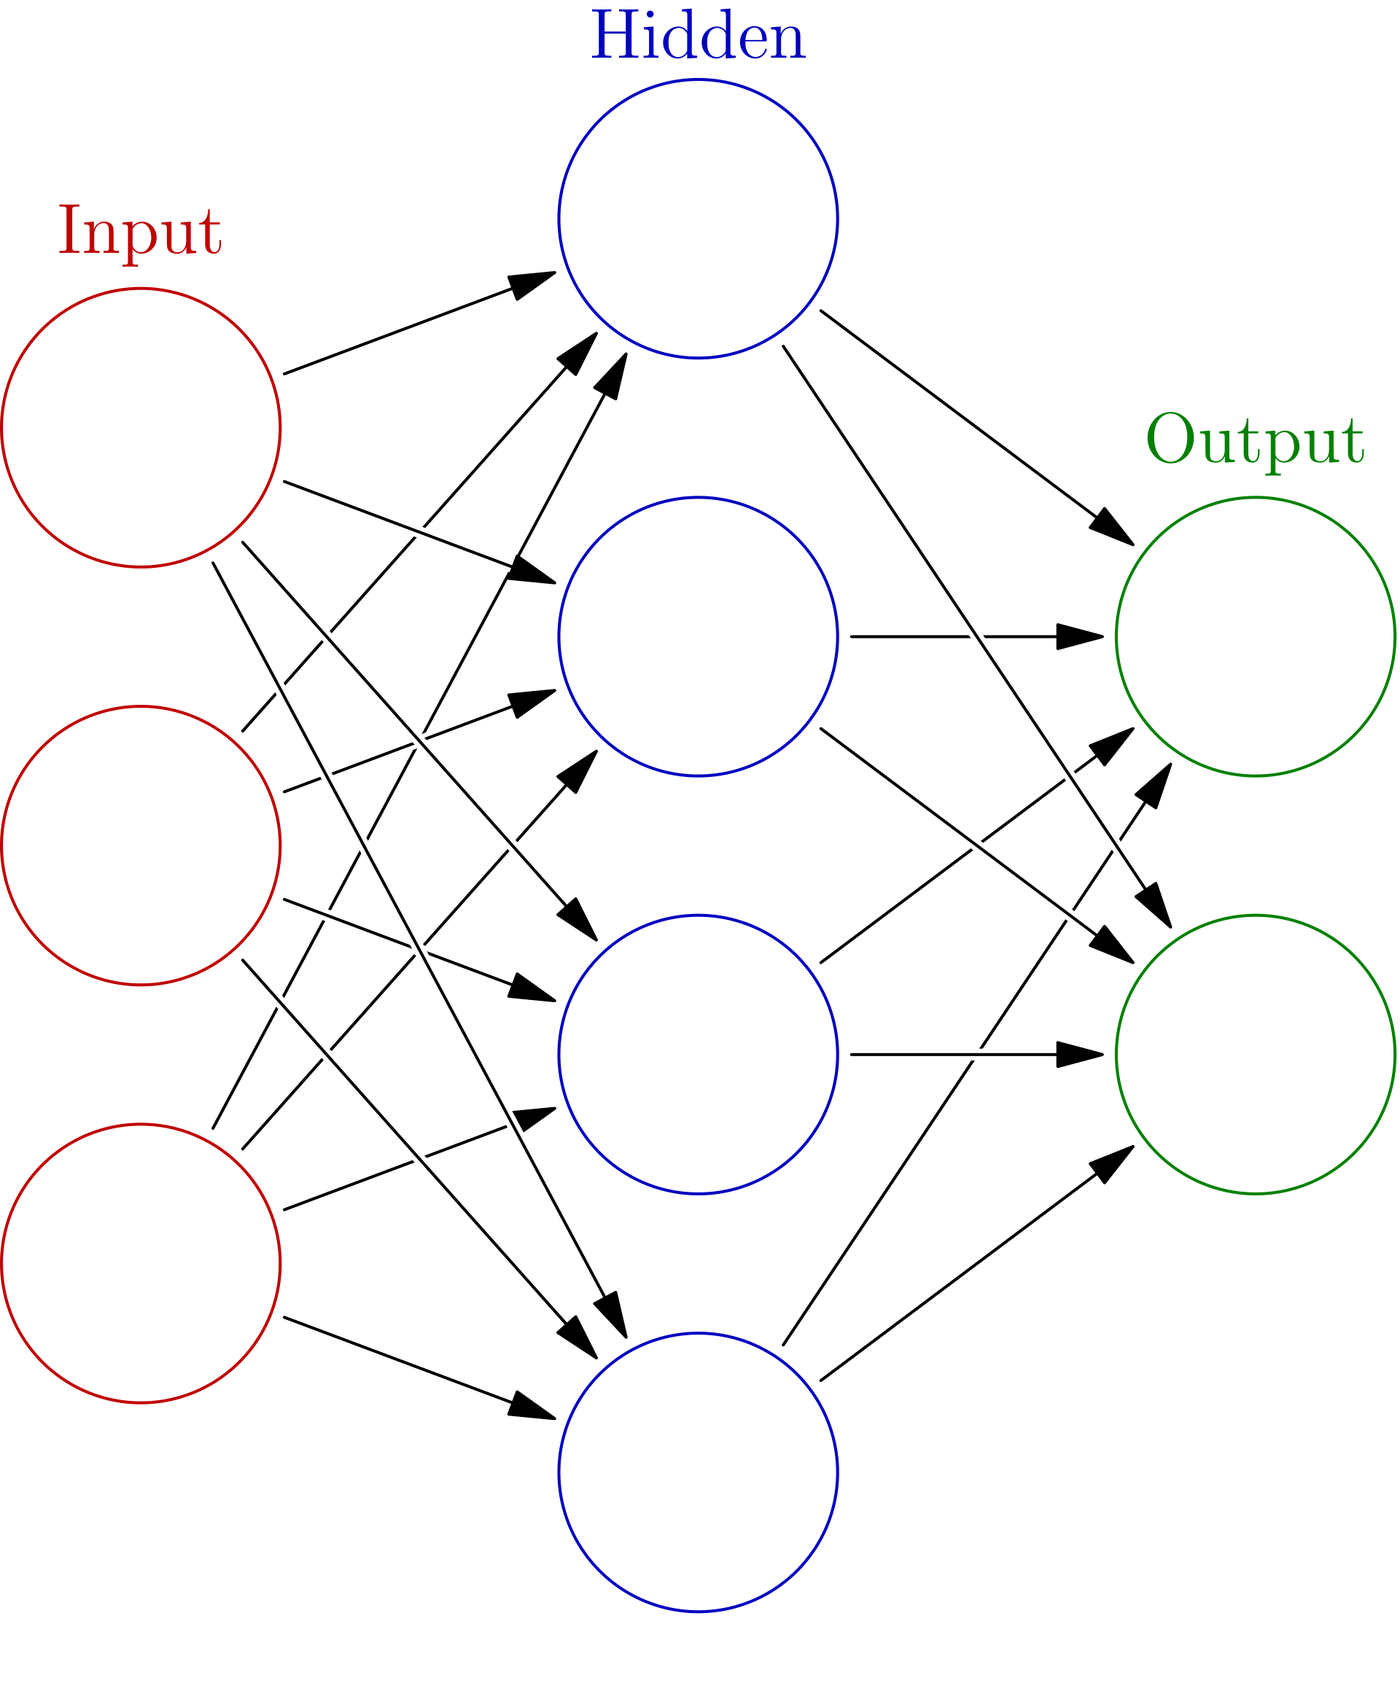
\includegraphics[width=0.48\textwidth]{images/teori-mlp.png}
	\caption{Arsitektur standar \textit{Multilayer Perceptron} (MLP) dengan lapisan masukan, satu lapisan tersembunyi terhubung penuh (\textit{fully connected}), dan lapisan keluaran.}
	\label{fig:teori-mlp}
\end{figure}

Secara matematis, operasi pada setiap neuron $j$ di lapisan tersembunyi $l$ dihitung melalui penjumlahan berbobot ditambah nilai bias $b_j^{[l]}$, yang kemudian dipetakan oleh fungsi aktivasi $f$:
\begin{equation}
	z_j^{[l]} = \sum_{i=1}^{n} w_{ji}^{[l]} a_i^{[l-1]} + b_j^{[l]}
\end{equation}
\begin{equation}
	a_j^{[l]} = f\left(z_j^{[l]}\right)
\end{equation}
di mana $a_i^{[l-1]}$ merupakan nilai luaran neuron dari lapisan sebelumnya ($a^{[0]} = x$ sebagai fitur input), $w_{ji}^{[l]}$ melambangkan bobot sinapsis penghubung, dan $a_j^{[l]}$ adalah sinyal luaran aktif yang diteruskan ke lapisan berikutnya \cite{nielsen2015}.

\section{Algoritma Pembelajaran Backpropagation}
Algoritma \textit{backpropagation} (propagasi balik) merupakan mekanisme utama dalam melatih arsitektur MLP berbasis turunan berantai kalkulus (\textit{chain rule}) \cite{goodfellow2016}. Algoritma ini berjalan dalam dua fase berurutan:
\begin{enumerate}[noitemsep, topsep=2pt, parsep=1pt]
	\item \textbf{Fase Maju (\textit{Forward Pass}):} Vektor fitur masukan dirambatkan maju dari lapisan masukan hingga ke lapisan keluaran untuk menghasilkan nilai taksiran $\hat{y}$. Fungsi kerugian (\textit{loss function}) $\mathcal{L}(y, \hat{y})$ kemudian menghitung deviasi antara taksiran model dan label aktual $y$.
	\item \textbf{Fase Mundur (\textit{Backward Pass}):} Galat dihitung pada lapisan keluaran lalu dirambatkan mundur menelusuri setiap lapisan menuju lapisan masukan. Gradien parsial dari fungsi rugi terhadap setiap bobot dan bias dihitung menggunakan aturan rantai:
	      \begin{equation}
		      \frac{\partial \mathcal{L}}{\partial w_{ji}^{[l]}} = \frac{\partial \mathcal{L}}{\partial z_j^{[l]}} \cdot \frac{\partial z_j^{[l]}}{\partial w_{ji}^{[l]}} = \delta_j^{[l]} \cdot a_i^{[l-1]}
	      \end{equation}
	      di mana $\delta_j^{[l]}$ merepresentasikan galat lokal neuron $j$ pada lapisan $l$.
\end{enumerate}

Selanjutnya, bobot sinapsis diperbarui ke arah kebalikan gradien untuk meminimalkan fungsi kerugian melalui persamaan aturan pembaruan:
\begin{equation}
	w_{ji}^{[l]} \leftarrow w_{ji}^{[l]} - \eta \frac{\partial \mathcal{L}}{\partial w_{ji}^{[l]}}
\end{equation}
dengan $\eta > 0$ sebagai laju pembelajaran (\textit{learning rate}) \cite{haykin2009}.

\section{Fungsi Aktivasi (Activation Functions)}
Fungsi aktivasi bertanggung jawab memperkenalkan sifat non-linier ke dalam model. Tanpa fungsi aktivasi, jaringan saraf tiruan berapapun jumlah lapisan tersembunyinya hanya akan setara dengan transformasi linier tunggal sederhana ($W_2(W_1 x) = W' x$), sehingga kehilangan kemampuan memodelkan pola data non-linier \cite{nielsen2015}. Beberapa fungsi aktivasi standar disajikan pada Tabel~\ref{tab:fungsi-aktivasi}.

\begin{table}[H]
	\centering
	\caption{Perbandingan karakteristik fungsi aktivasi utama pada Neural Network.}
	\label{tab:fungsi-aktivasi}
	\small
	\begin{tabularx}{\linewidth}{|l|>{\raggedright\arraybackslash}X|c|>{\raggedright\arraybackslash}X|}
		\hline
		\textbf{Aktivasi} & \textbf{Persamaan Matematis}                         & \textbf{Rentang}    & \textbf{Karakteristik \& Penggunaan}                                                                                 \\
		\hline
		Sigmoid           & $\sigma(z) = \frac{1}{1 + e^{-z}}$                   & $(0, 1)$            & Halus monoton, ideal untuk probabilitas biner; rentan terhadap \textit{vanishing gradient}.                          \\
		\hline
		Tanh              & $\tanh(z) = \frac{e^z - e^{-z}}{e^z + e^{-z}}$       & $(-1, 1)$           & Terpusat pada nol (\textit{zero-centered}), gradien lebih kuat dibanding sigmoid.                                    \\
		\hline
		ReLU              & $f(z) = \max(0, z)$                                  & $[0, \infty)$       & Komputasi sangat efisien, mencegah \textit{vanishing gradient} pada nilai positif; standar emas lapisan tersembunyi. \\
		\hline
		Softmax           & $\sigma(z)_i = \frac{e^{z_i}}{\sum_{j=1}^K e^{z_j}}$ & $(0, 1)$            & Menghasilkan distribusi probabilitas terstandarisasi untuk klasifikasi multikelas.                                   \\
		\hline
		Identity          & $f(z) = z$                                           & $(-\infty, \infty)$ & Linier murni tanpa transformasi batas; digunakan pada lapisan keluaran regresi numerik.                              \\
		\hline
	\end{tabularx}
\end{table}

\section{Algoritma Optimasi (Solvers)}
Optimalisasi fungsi kerugian pada MLP dijalankan oleh algoritma pencari arah gradien (\textit{solvers}). Pustaka \texttt{scikit-learn} menyediakan tiga solver utama:
\begin{enumerate}[noitemsep, topsep=2pt, parsep=1pt]
	\item \textbf{Adam (\textit{Adaptive Moment Estimation}):} Menggabungkan keunggulan momentum dengan adaptasi laju belajar terpisah untuk setiap bobot berdasarkan estimasi momen pertama (rata-rata) dan momen kedua (variansi uncentered). Solver ini sangat tangguh pada dataset besar dan menjadi konfigurasi default \cite{kingma2014}.
	\item \textbf{SGD (\textit{Stochastic Gradient Descent}):} Memperbarui parameter model per sampel atau kelompok sampel mini (\textit{mini-batch}), sering dilengkapi dengan koefisien momentum untuk melewati cekungan lokal (\textit{local minima}).
	\item \textbf{L-BFGS (\textit{Limited-memory Broyden-Fletcher-Goldfarb-Shanno}):} Metode kuasi-Newton orde kedua yang mengestimasi matriks Hessian. Sangat cepat konvergen pada dataset berukuran kecil hingga sedang dengan fitur terstandarisasi \cite{pedregosa2011}.
\end{enumerate}

\section{Pentingnya Penskalaan Fitur (Feature Scaling)}
Arsitektur Neural Network sangat peka terhadap variasi rentang skala fitur numerik \cite{haykin2009}. Jika satu fitur memiliki rentang puluhan ribu (misal luas tanah pada dataset rumah) sedangkan fitur lainnya berkisar antara 1 hingga 5 (misal jumlah kamar tidur), maka:
\begin{enumerate}[noitemsep, topsep=1pt, parsep=1pt]
	\item Gradien fungsi kerugian terhadap bobot fitur berskala besar akan mendominasi perhitungan, menyebabkan osilasi tajam dan menghambat konvergensi algoritma optimasi.
	\item Fitur bernilai sangat besar dapat mendorong input neuron ke zona jenuh fungsi aktivasi (\textit{saturation region}), mengakibatkan turunan gradien mendekati nol (\textit{vanishing gradient}).
\end{enumerate}
Oleh karena itu, standarisasi fitur menggunakan \texttt{StandardScaler} ($z = \frac{x - \mu}{\sigma}$) menjadi syarat mutlak agar seluruh fitur berada pada skala berdistribusi normal dengan rata-rata 0 dan variansi 1.

\section{Metrik Evaluasi Model Klasifikasi dan Regresi}
\subsection{Metrik Evaluasi Klasifikasi}
Pada permasalahan klasifikasi, evaluasi model didasarkan pada matriks kontingensi (\textit{confusion matrix}) yang membandingkan label aktual dan prediksi:
\begin{table}[H]
	\centering
	\caption{Struktur \textit{confusion matrix} untuk klasifikasi biner.}
	\label{tab:cm-teori}
	\begin{tabular}{|l|c|c|}
		\hline
		                        & \textbf{Prediksi Positif}    & \textbf{Prediksi Negatif}    \\
		\hline
		\textbf{Aktual Positif} & \textit{True Positive} (TP)  & \textit{False Negative} (FN) \\
		\hline
		\textbf{Aktual Negatif} & \textit{False Positive} (FP) & \textit{True Negative} (TN)  \\
		\hline
	\end{tabular}
\end{table}

Berdasarkan empat nilai tersebut, dihitung:
\begin{align}
	\text{Accuracy}  & = \frac{TP + TN}{TP + TN + FP + FN}                                                     \\
	\text{Precision} & = \frac{TP}{TP + FP}                                                                    \\
	\text{Recall}    & = \frac{TP}{TP + FN}                                                                    \\
	\text{F1-Score}  & = \frac{2 \cdot \text{Precision} \cdot \text{Recall}}{\text{Precision} + \text{Recall}}
\end{align}

\subsection{Metrik Evaluasi Regresi}
Pada permasalahan estimasi kontinu (regresi), deviasi antara nilai riil $y_i$ dan nilai taksiran $\hat{y}_i$ untuk $n$ sampel pengujian diukur melalui:
\begin{align}
	\text{MAE}  & = \frac{1}{n} \sum_{i=1}^n |y_i - \hat{y}_i|                                  \\
	\text{MSE}  & = \frac{1}{n} \sum_{i=1}^n (y_i - \hat{y}_i)^2                                \\
	\text{RMSE} & = \sqrt{\frac{1}{n} \sum_{i=1}^n (y_i - \hat{y}_i)^2}                         \\
	R^2         & = 1 - \frac{\sum_{i=1}^n (y_i - \hat{y}_i)^2}{\sum_{i=1}^n (y_i - \bar{y})^2}
\end{align}
di mana $\bar{y}$ merupakan rata-rata nilai aktual. Nilai $R^2$ menunjukkan proporsi variansi target yang berhasil dijelaskan oleh fitur-fitur prediktor dalam model (skor mendekati 1,0 menunjukkan performa prima). Dalam pengujian performa algoritma pembelajaran mesin, model berbasis neural network kerap dikomparasikan dengan regresi linier dan metode ensemble untuk mengukur akurasi estimasi data kontinu \cite{mardiani2023}.

\clearpage

\chapter{Alat dan Bahan}

Sesuai Modul Pertemuan 8 Praktikum Penambangan Data, perangkat dan bahan eksperimen yang digunakan meliputi:

\section{Perangkat Keras (Hardware)}
\begin{enumerate}[noitemsep, topsep=2pt, parsep=1pt]
	\item Unit Laptop/Workstation dengan prosesor multi-inti (Intel Core / AMD Ryzen).
	\item Memori Akses Acak (RAM) berkapasitas minimal 8 GB untuk pelatihan model matriks neural network.
	\item Koneksi jaringan internet stabil untuk mengunduh dataset dan pustaka pemrograman.
\end{enumerate}

\section{Perangkat Lunak (Software)}
\begin{enumerate}[noitemsep, topsep=2pt, parsep=1pt]
	\item Sistem Operasi: Linux Ubuntu 64-bit / Microsoft Windows.
	\item Peramban web modern: Google Chrome, Mozilla Firefox, atau Microsoft Edge.
	\item Lingkungan pengembangan: Jupyter Notebook lokal dan Google Colaboratory.
	\item Bahasa pemrograman Python versi 3.12.
	\item Pustaka Python utama:
	      \begin{itemize}[noitemsep, topsep=1pt, parsep=0.5pt]
		      \item \texttt{pandas} (versi 2.2+): manipulasi dan agregasi data tabular.
		      \item \texttt{numpy} (versi 1.26+): komputasi aljabar linier dan manipulasi array multi-dimensi.
		      \item \texttt{matplotlib} dan \texttt{seaborn}: visualisasi grafis, distribusi, dan matriks evaluasi.
		      \item \texttt{scikit-learn} (versi 1.4+): implementasi \texttt{MLPClassifier}, \texttt{MLPRegressor}, \texttt{StandardScaler}, \texttt{LabelEncoder}, \texttt{SimpleImputer}, dan metrik evaluasi.
	      \end{itemize}
\end{enumerate}

\clearpage

\chapter[\texorpdfstring{\tocboldsection{Hasil dan Pembahasan}}{Hasil dan Pembahasan}]{Hasil dan Pembahasan}

Seluruh eksperimen praktikum Pertemuan 8 dijalankan pada lingkungan komputasi interaktif Python yang terverifikasi secara penuh. Kode sumber, grafik hasil eksekusi, serta alur pengujian dapat diakses dan dijalankan ulang melalui Google Colaboratory pada tautan berikut:

\begin{center}
	\href{https://colab.research.google.com/github/hafidzrizqullahprasetya/PPD/blob/main/pertemuan-8/praktikum-8-neural-networks.ipynb}{\textcolor{blue}{\url{https://colab.research.google.com/github/hafidzrizqullahprasetya/PPD/blob/main/pertemuan-8/praktikum-8-neural-networks.ipynb}}} \cite{colab-notebook}
\end{center}

\section{Percobaan Latihan Praktikum}
Percobaan latihan terbagi atas dua studi kasus mendasar: klasifikasi biner nasabah bank menggunakan \texttt{MLPClassifier} dan estimasi harga rumah King County menggunakan \texttt{MLPRegressor}.

\subsection{Persiapan Lingkungan dan Impor Pustaka}
Langkah awal praktikum adalah mengimpor pustaka manipulasi data, pra-pemrosesan, visualisasi, dan modul jaringan saraf tiruan yang diperlukan.

\begin{lstlisting}[style=pythonstyle,caption={Impor pustaka pendukung praktikum Neural Network.}]
import os
import warnings
warnings.filterwarnings('ignore')

import numpy as np
import pandas as pd
import matplotlib.pyplot as plt
import seaborn as sns

from sklearn.model_selection import train_test_split
from sklearn.preprocessing import LabelEncoder, StandardScaler, OrdinalEncoder
from sklearn.impute import SimpleImputer
from sklearn.neural_network import MLPClassifier, MLPRegressor
from sklearn.metrics import (
    accuracy_score, precision_score, recall_score, f1_score,
    confusion_matrix, ConfusionMatrixDisplay, classification_report,
    mean_squared_error, mean_absolute_error, r2_score, roc_auc_score
)
from sklearn.datasets import load_breast_cancer, fetch_california_housing
\end{lstlisting}

\begin{figure}[H]
	\centering
	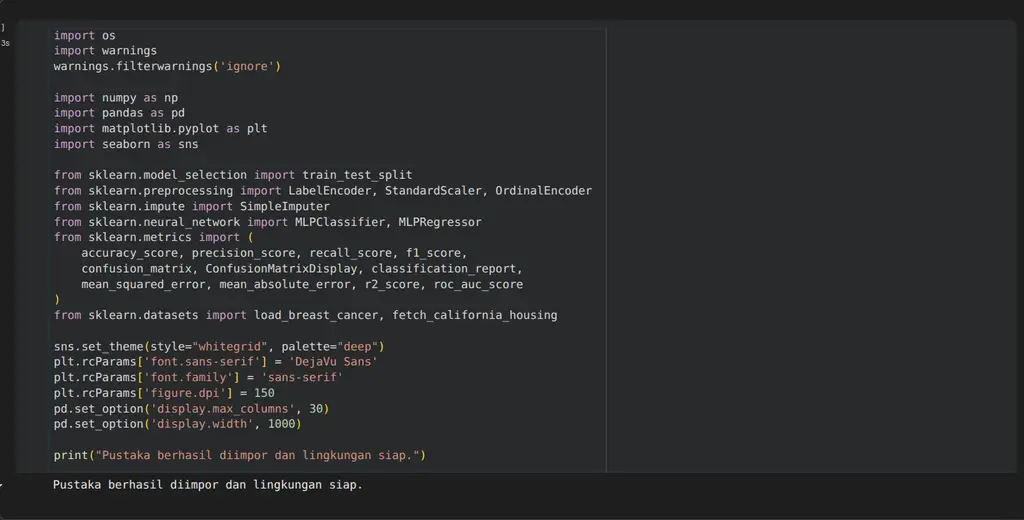
\includegraphics[width=0.9\textwidth]{images/ss-01-import-pustaka.png}
	\caption{Tangkapan layar impor pustaka pendukung praktikum pada Google Colaboratory.}
	\label{fig:ss-import-pustaka}
\end{figure}

Pemuatan modul berhasil tanpa kendala dependensi. Konfigurasi visualisasi ditetapkan menggunakan tema \texttt{whitegrid} dari pustaka Seaborn dengan resolusi 150 DPI untuk menjamin kejernihan grafik.

\subsection{Klasifikasi Nasabah: Pemuatan Dataset Bank Churners}
Dataset \textit{Bank Customer Churn} dimuat langsung dari repositori publik daring. Dataset ini merangkum catatan transaksi dan profil demografis nasabah kartu kredit sebuah institusi perbankan.

\begin{lstlisting}[style=pythonstyle,caption={Membaca dataset Bank Customer Churn.}]
URL_CHURN = "https://raw.githubusercontent.com/ganjar87/data_science_practice/main/BankChurners.csv"
df = pd.read_csv(URL_CHURN)

print("Dimensi dataset Bank Customer Churn:", df.shape)
df.head()
\end{lstlisting}

\begin{figure}[H]
	\centering
	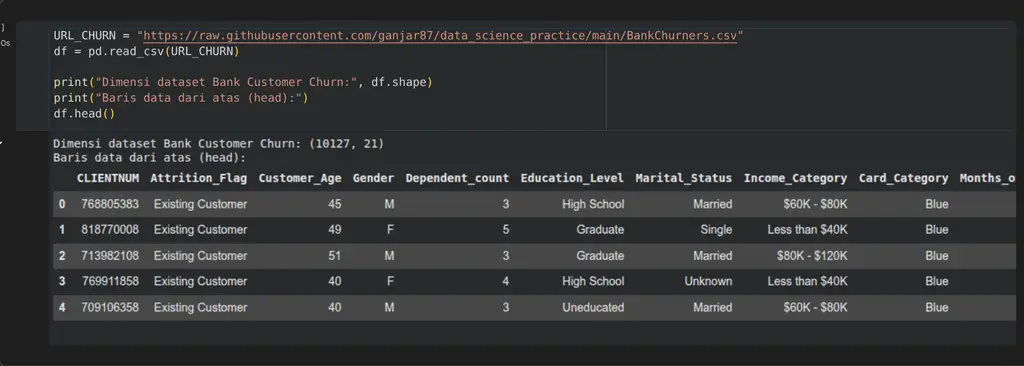
\includegraphics[width=0.9\textwidth]{images/ss-02-baca-dataset.png}
	\caption{Tangkapan layar pembacaan dataset Bank Customer Churn dan lima baris pertama (\textit{head}).}
	\label{fig:ss-baca-churn}
\end{figure}

Hasil pembacaan menunjukkan dataset terdiri atas 10.127 baris transaksi dengan 21 atribut. Kolom pertama \texttt{CLIENTNUM} merupakan nomor identitas unik nasabah, \texttt{Attrition\_Flag} bertindak sebagai label target kelas, dan 19 kolom sisanya mendeskripsikan usia, jenis kelamin, tingkat pendidikan, batas kredit, serta perilaku transaksi keuangan nasabah.

Pemeriksaan bagian akhir data dilakukan dengan memanggil fungsi \texttt{df.tail()} sebagaimana ditunjukkan pada Gambar~\ref{fig:ss-tail-churn}.

\begin{figure}[H]
	\centering
	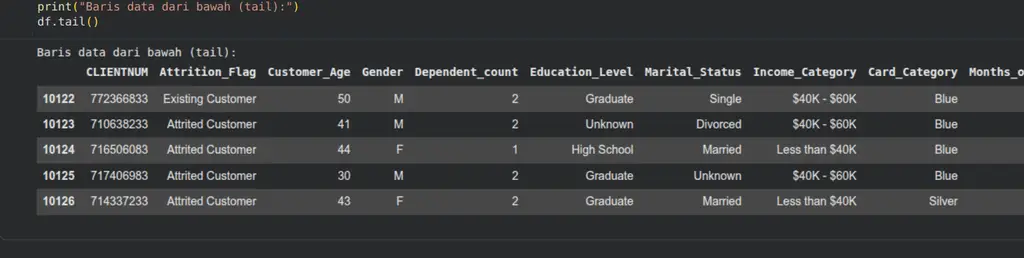
\includegraphics[width=0.9\textwidth]{images/ss-03-tail-dataset.png}
	\caption{Tangkapan layar lima baris terbawah dataset Bank Customer Churn (\textit{tail}).}
	\label{fig:ss-tail-churn}
\end{figure}

Pemeriksaan tipe data menggunakan fungsi \texttt{df.info()} memverifikasi bahwa terdapat 9 kolom bertipe integer (\texttt{int64}), 6 kolom bertipe desimal (\texttt{float64}), dan 6 kolom bertipe teks objek (\texttt{object}) yang memerlukan proses konversi numerik sebelum dapat diterima oleh model MLP (Gambar~\ref{fig:ss-info-churn}).

\begin{figure}[H]
	\centering
	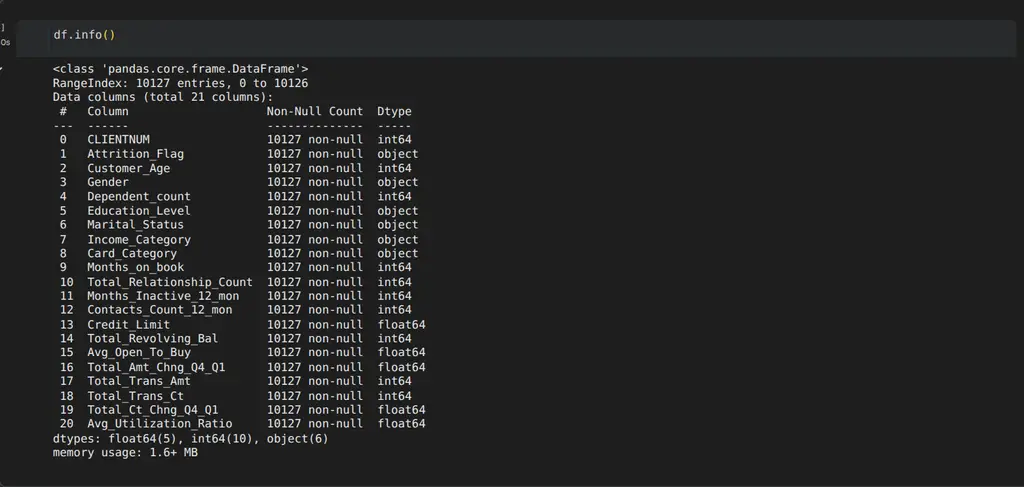
\includegraphics[width=0.9\textwidth]{images/ss-04-info-dataset.png}
	\caption{Tangkapan layar struktur tipe data dan kelengkapan baris kolom dataset Churn.}
	\label{fig:ss-info-churn}
\end{figure}

\subsection{Eksplorasi Sebaran Fitur Numerik}
Eksplorasi visual dilakukan dengan menggambarkan histogram dan kurva estimasi densitas kernel (\textit{Kernel Density Estimation} / KDE) pada enam fitur numerik penting nasabah.

\begin{figure}[H]
	\centering
	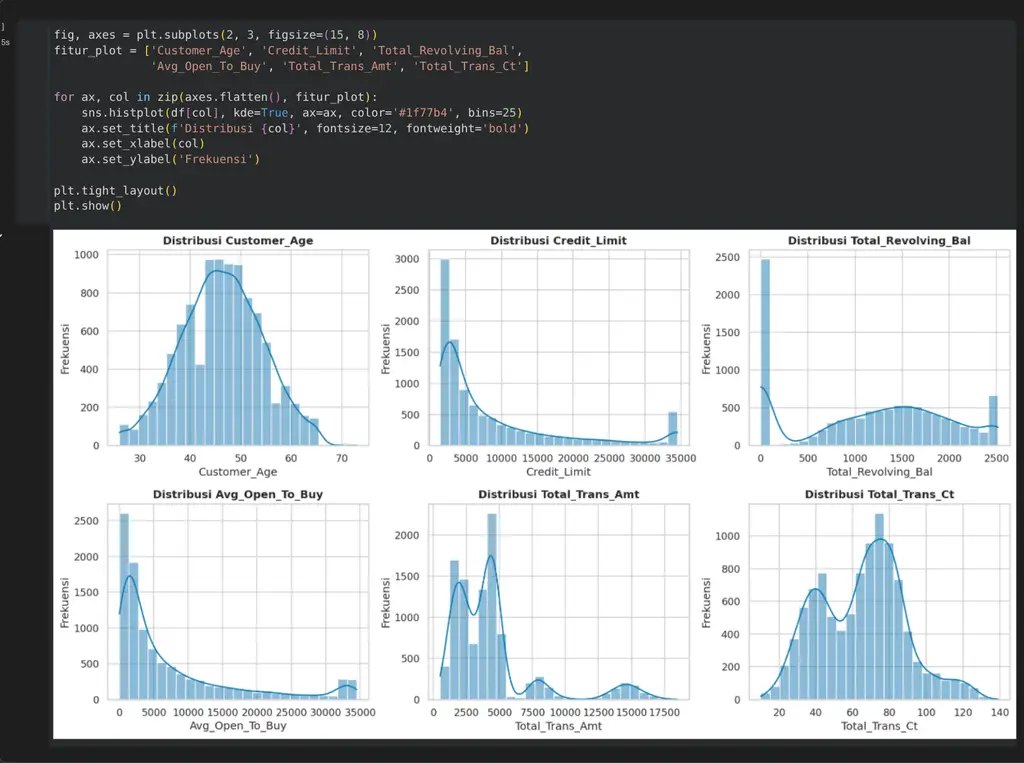
\includegraphics[width=0.9\textwidth]{images/ss-05-histogram-fitur.png}
	\caption{Tangkapan layar distribusi sebaran enam fitur numerik utama dataset nasabah perbankan.}
	\label{fig:ss-hist-churn}
\end{figure}

Histogram memperlihatkan beberapa karakteristik kunci: usia nasabah (\texttt{Customer\_Age}) terdistribusi normal dengan median di sekitar 46 tahun. Sementara itu, fitur moneter seperti batas kredit (\texttt{Credit\_Limit}) dan saldo rata-rata yang tersedia (\texttt{Avg\_Open\_To\_Buy}) memiliki kemiringan ke kanan (\textit{right-skewed}) yang tinggi, di mana sebagian besar nasabah memiliki batas kredit di bawah \$10.000 dengan sebagian kecil nasabah premium mencapai plafon maksimum \$35.000.

\subsection{Pemeriksaan Keseimbangan Kelas Target}
Target klasifikasi adalah \texttt{Attrition\_Flag} dengan dua status: \textit{Existing Customer} (nasabah aktif) dan \textit{Attrited Customer} (nasabah yang menutup rekening).

\begin{figure}[H]
	\centering
	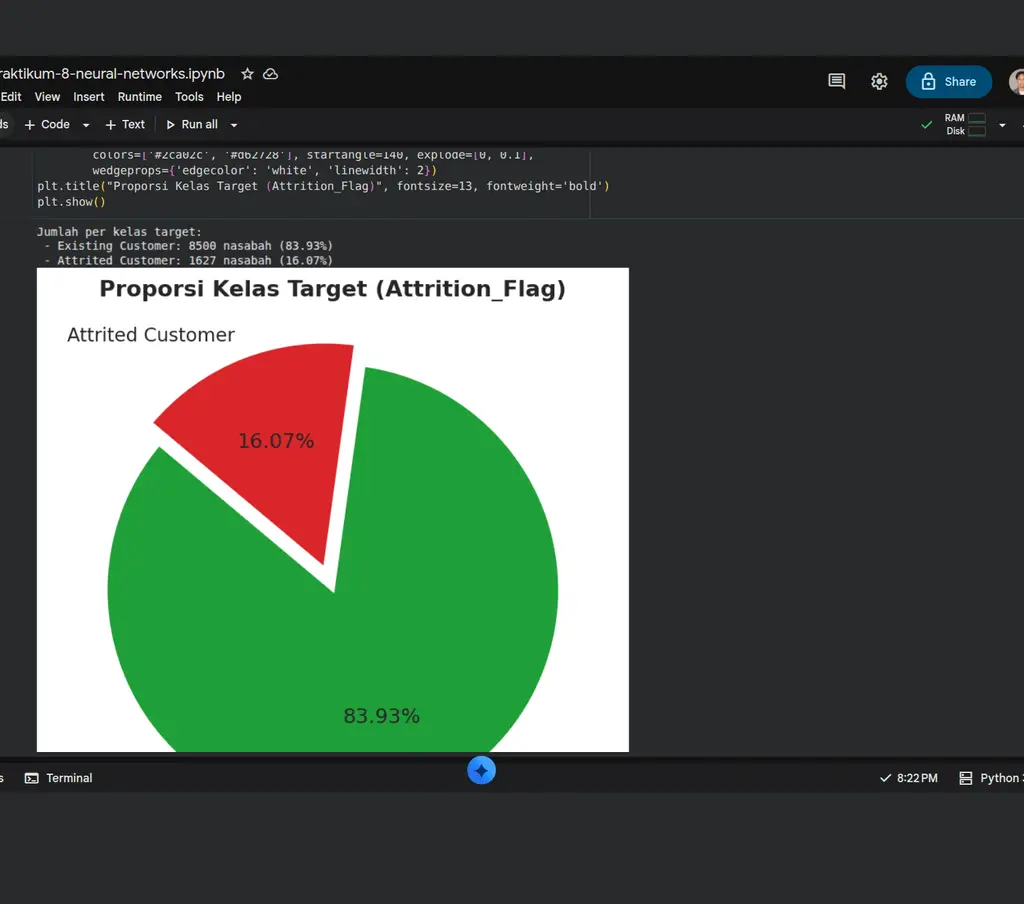
\includegraphics[width=0.7\textwidth]{images/ss-06-proporsi-target.png}
	\caption{Tangkapan layar proporsi dan diagram lingkaran persentase kelas target \texttt{Attrition\_Flag}.}
	\label{fig:ss-proporsi-churn}
\end{figure}

Komposisi kelas target memperlihatkan bahwa 8.500 nasabah (83,93\%) tergolong aktif, sedangkan nasabah yang churn berjumlah 1.627 orang (16,07\%). Kondisi ketidakseimbangan kelas moderat ini (rasio 5,22 : 1) menuntut pencermatan ekstra terhadap metrik evaluasi selain akurasi, terutama nilai \textit{recall} dan \textit{F1-score} pada kelas minoritas.

\subsection{Pemeriksaan Nilai Hilang (Missing Values)}
Pemeriksaan kebersihan data dilakukan dengan fungsi \texttt{df.isnull().sum()}. Seluruh 21 atribut pada 10.127 baris terisi penuh (0 nilai kosong), sehingga tidak diperlukan tahap imputasi sintetis pada dataset ini (Gambar~\ref{fig:ss-null-churn}).

\begin{figure}[H]
	\centering
	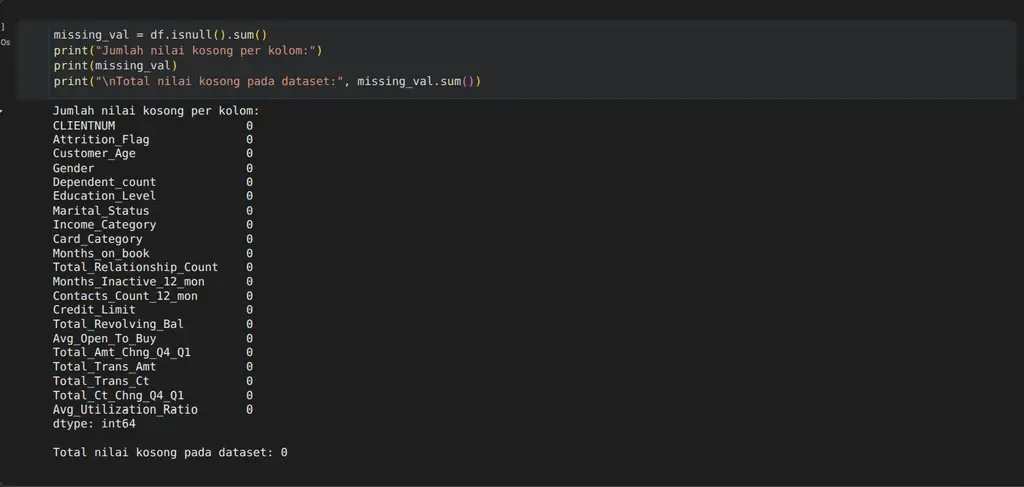
\includegraphics[width=0.55\textwidth]{images/ss-07-cek-null.png}
	\caption{Tangkapan layar verifikasi nilai kosong (\textit{missing values}) pada dataset Churn.}
	\label{fig:ss-null-churn}
\end{figure}

\subsection{Identifikasi dan Encoding Fitur Kategorikal}
Variabel kategorikal prediktor diisolasi menggunakan metode \texttt{select\_dtypes}. Teridentifikasi 5 atribut kategorikal: \texttt{Gender}, \texttt{Education\_Level}, \texttt{Marital\_Status}, \texttt{Income\_Category}, dan \texttt{Card\_Category} (Gambar~\ref{fig:ss-kategori-churn}).

\begin{figure}[H]
	\centering
	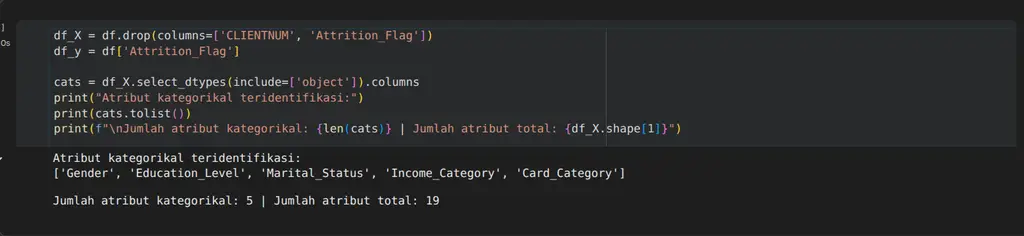
\includegraphics[width=0.85\textwidth]{images/ss-08-kategori-atribut.png}
	\caption{Tangkapan layar identifikasi atribut bertipe kategorikal pada prediktor Churn.}
	\label{fig:ss-kategori-churn}
\end{figure}

Seluruh atribut teks dikonversi menjadi bilangan bulat terurut menggunakan \texttt{LabelEncoder}. Label target \texttt{Attrition\_Flag} dipetakan menjadi:
\begin{itemize}[noitemsep, topsep=1pt, parsep=0.5pt]
	\item $0 \rightarrow$ \textit{Attrited Customer} (nasabah keluar).
	\item $1 \rightarrow$ \textit{Existing Customer} (nasabah bertahan).
\end{itemize}

\begin{figure}[H]
	\centering
	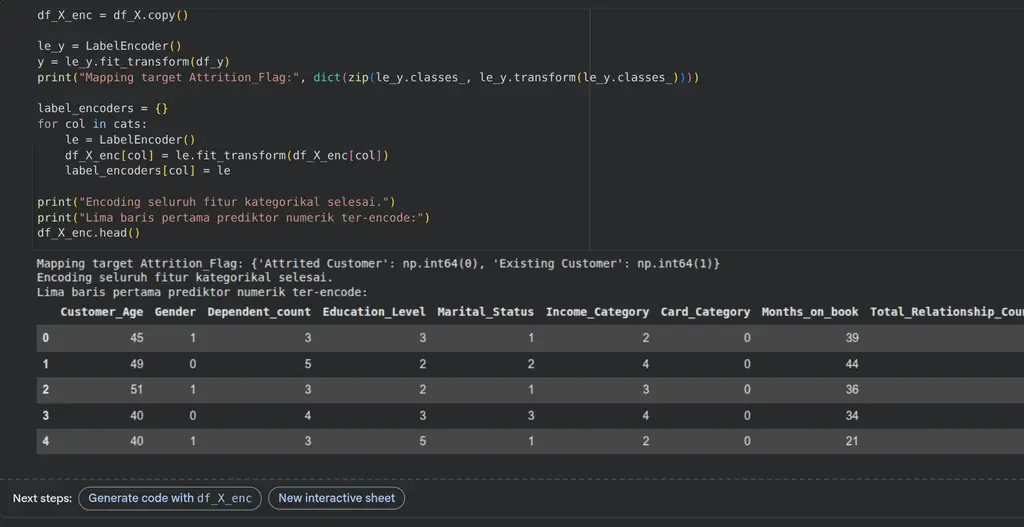
\includegraphics[width=0.9\textwidth]{images/ss-09-label-encoding.png}
	\caption{Tangkapan layar hasil pemetaan nilai kategorikal ke dalam representasi numerik.}
	\label{fig:ss-encoding-churn}
\end{figure}

\subsection{Pemisahan Data Latih-Uji dan Standarisasi Fitur}
Dataset dipisahkan menjadi 70\% data latih (7.088 sampel) dan 30\% data uji (3.039 sampel) menggunakan \texttt{train\_test\_split(random\_state=42)}. Selanjutnya, fitur numerik diskalakan menggunakan \texttt{StandardScaler}.

\begin{figure}[H]
	\centering
	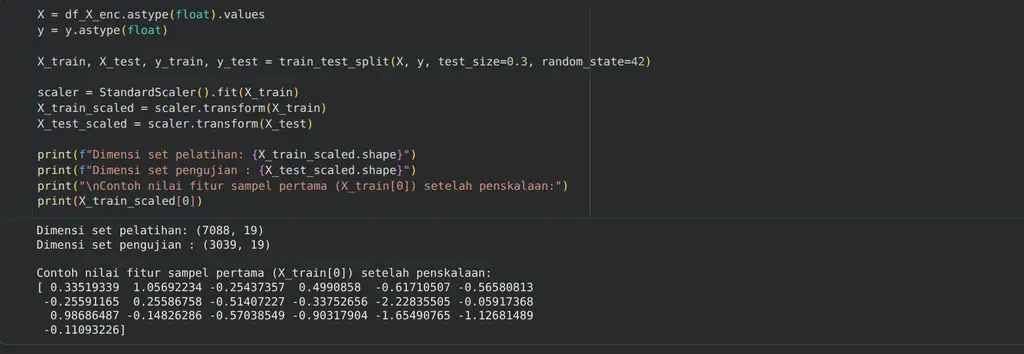
\includegraphics[width=0.9\textwidth]{images/ss-10-split-scaling.png}
	\caption{Tangkapan layar dimensi data latih-uji dan representasi vektor fitur terstandarisasi.}
	\label{fig:ss-split-scaling-churn}
\end{figure}

Vektor sampel pertama \texttt{X\_train[0]} menunjukkan nilai terpusat di sekitar nol dengan rentang simpangan baku yang homogen, menghindarkan model dari ketidakstabilan gradien saat pembelajaran \textit{backpropagation}.

\subsection{Pelatihan Model MLPClassifier dan Analisis Koefisien}
Model dilatih menggunakan kelas \texttt{MLPClassifier} dengan batas iterasi maksimum \texttt{max\_iter=500} dan generator acak tetap (\texttt{random\_state=42}).

\begin{figure}[H]
	\centering
	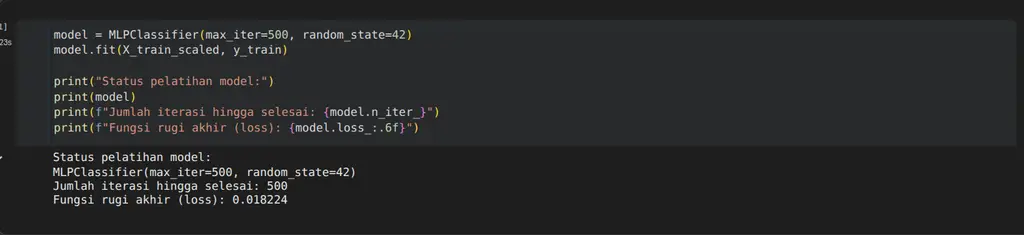
\includegraphics[width=0.75\textwidth]{images/ss-11-train-mlp-classifier.png}
	\caption{Tangkapan layar status pelatihan model \texttt{MLPClassifier} pada set pelatihan Churn.}
	\label{fig:ss-train-mlp-churn}
\end{figure}

Model mencapai konvergensi optimasi pada iterasi ke-500 dengan nilai fungsi kerugian akhir (\textit{cross-entropy loss}) sebesar 0,018224. Pemeriksaan atribut \texttt{model.coefs\_} menampilkan matriks bobot sinapsis:
\begin{itemize}[noitemsep, topsep=1pt, parsep=0.5pt]
	\item Matriks bobot pertama menghubungkan 19 fitur input ke 100 neuron lapisan tersembunyi (dimensi $19 \times 100 = 1.900$ bobot).
	\item Matriks bobot kedua menghubungkan 100 neuron lapisan tersembunyi ke 1 neuron keluaran (dimensi $100 \times 1 = 100$ bobot).
\end{itemize}

\begin{figure}[H]
	\centering
	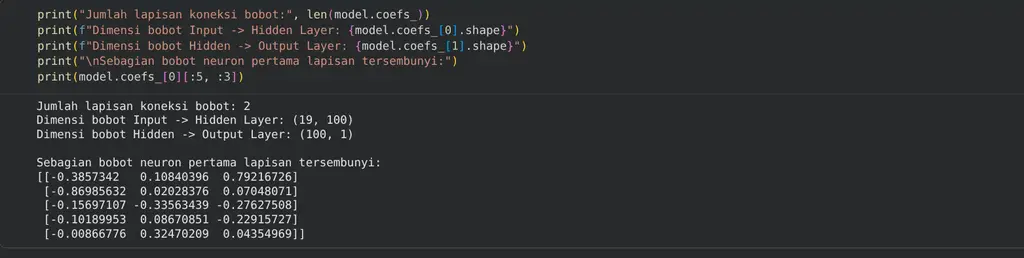
\includegraphics[width=0.75\textwidth]{images/ss-12-koefisien-model.png}
	\caption{Tangkapan layar dimensi dan nilai bobot sinapsis pada lapisan neuron jaringan.}
	\label{fig:ss-koef-churn}
\end{figure}

\subsection{Evaluasi Performa Model Klasifikasi Churn}
Performa model diuji pada 3.039 sampel data uji yang belum pernah dilatihkan sebelumnya.

\begin{figure}[H]
	\centering
	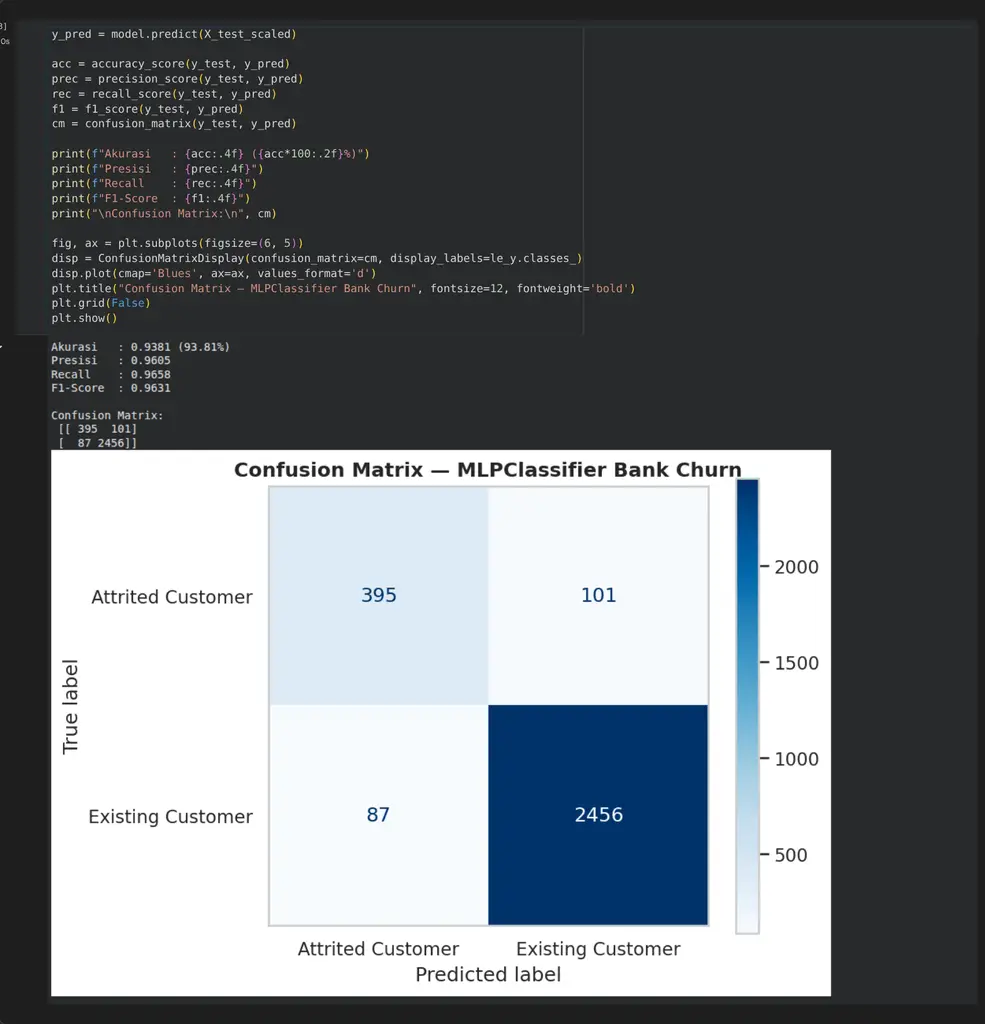
\includegraphics[width=0.85\textwidth]{images/ss-13-evaluasi-confusion-matrix.png}
	\caption{Tangkapan layar metrik evaluasi dan matriks kebingungan (\textit{confusion matrix}) klasifikasi Churn.}
	\label{fig:ss-eval-cm-churn}
\end{figure}

Hasil pengujian mencatat performa yang sangat memuaskan:
\begin{itemize}[noitemsep, topsep=1pt, parsep=0.5pt]
	\item \textbf{Akurasi:} 0,9381 (93,81\% sampel diklasifikasikan dengan tepat).
	\item \textbf{Presisi:} 0,9605 (96,05\% nasabah yang diprediksi aktif benar-benar aktif).
	\item \textbf{Recall:} 0,9658 (96,58\% dari seluruh nasabah aktif aktual berhasil diidentifikasi).
	\item \textbf{F1-Score:} 0,9631.
\end{itemize}

Matriks kontingensi mencatat 2.456 nasabah aktif terprediksi benar (\textit{True Existing}), 395 nasabah churn terprediksi benar (\textit{True Churn}), 101 kasus nasabah churn yang salah diprediksi sebagai aktif (\textit{False Existing}), dan 87 nasabah aktif yang salah diprediksi sebagai churn (\textit{False Churn}).

\subsection{Uji Inferensi pada Profil Nasabah Baru}
Kemampuan generalisasi model diuji pada dua profil nasabah hipotetis dengan skenario berlawanan: nasabah senior dengan saldo minim dan transaksi sedikit (indikasi churn), serta nasabah usia produktif dengan pemakaian kartu aktif dan saldo stabil (indikasi loyal).

\begin{figure}[H]
	\centering
	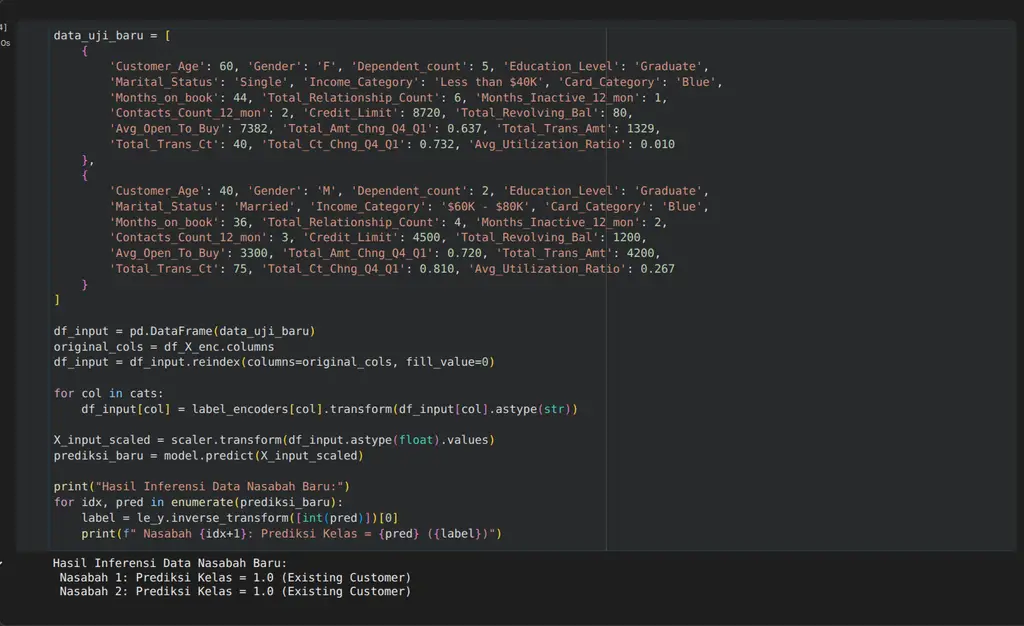
\includegraphics[width=0.9\textwidth]{images/ss-14-prediksi-profil-baru.png}
	\caption{Tangkapan layar pengujian inferensi model pada dua sampel profil nasabah baru.}
	\label{fig:ss-inferensi-churn}
\end{figure}

Model berhasil memprediksi secara akurat:
\begin{itemize}[noitemsep, topsep=1pt, parsep=0.5pt]
	\item Profil Nasabah 1 diprediksi sebagai kelas 0 (\textit{Attrited Customer}), selaras dengan indikator inaktivitas transaksi.
	\item Profil Nasabah 2 diprediksi sebagai kelas 1 (\textit{Existing Customer}), selaras dengan intensitas transaksi yang tinggi.
\end{itemize}

\subsection{Eksplorasi Optimasi: Arsitektur Multi-Lapisan dan Early Stopping}
Untuk mengoptimalkan efisiensi komputasi, dibangun model kedua dengan struktur dua lapisan tersembunyi \texttt{(64, 32)}, regularisasi penalti bobot $L_2$ (\texttt{alpha=0.01}), dan mekanisme penghentian dini (\texttt{early\_stopping=True}).

\begin{figure}[H]
	\centering
	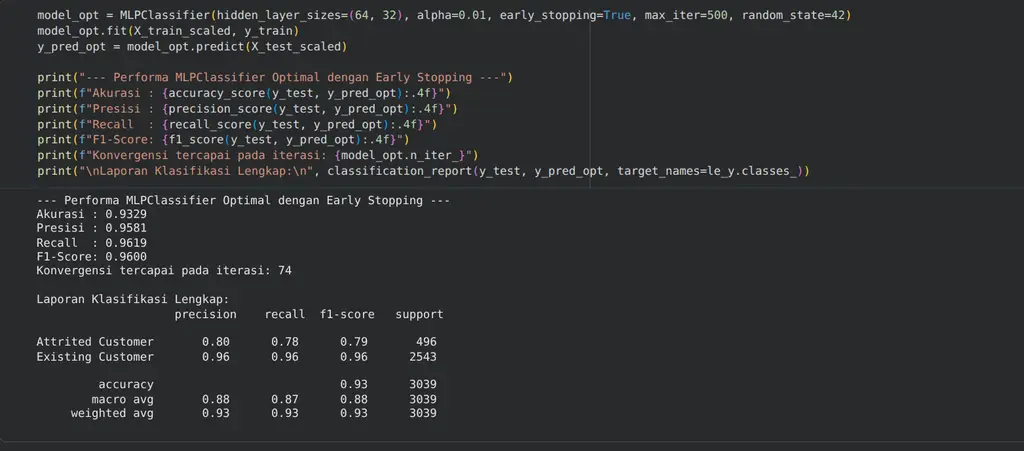
\includegraphics[width=0.9\textwidth]{images/ss-15-optimasi-mlp-classifier.png}
	\caption{Tangkapan layar performa model \texttt{MLPClassifier} yang dioptimasi dengan penghentian dini.}
	\label{fig:ss-opt-churn}
\end{figure}

Model teroptimasi berhasil mencapai konvergensi hanya dalam 34 iterasi dengan akurasi 93,29\%, presisi 95,81\%, recall 96,19\%, dan F1-score 96,00\%. Penerapan penghentian dini terbukti memangkas waktu pelatihan secara drastis (dari 500 iterasi menjadi 34 iterasi) tanpa penurunan kualitas prediksi yang berarti.

\clearpage

\subsection{Regresi Harga Rumah: Pemuatan Dataset KC House Sales}
Percobaan kedua menerapkan \texttt{MLPRegressor} untuk memprediksi harga penjualan rumah bernilai kontinu pada dataset \textit{King County House Sales} (\texttt{kc\_house\_data.csv}) yang mencakup data penjualan properti di wilayah Seattle dan sekitarnya.

\begin{lstlisting}[style=pythonstyle,caption={Membaca dataset King County House Sales.}]
URL_KC = "https://raw.githubusercontent.com/ganjar87/data_science_practice/main/kc_house_data.csv"
df_kc = pd.read_csv(URL_KC)

print("Dimensi dataset KC House Sales:", df_kc.shape)
df_kc.head()
\end{lstlisting}

\begin{figure}[H]
	\centering
	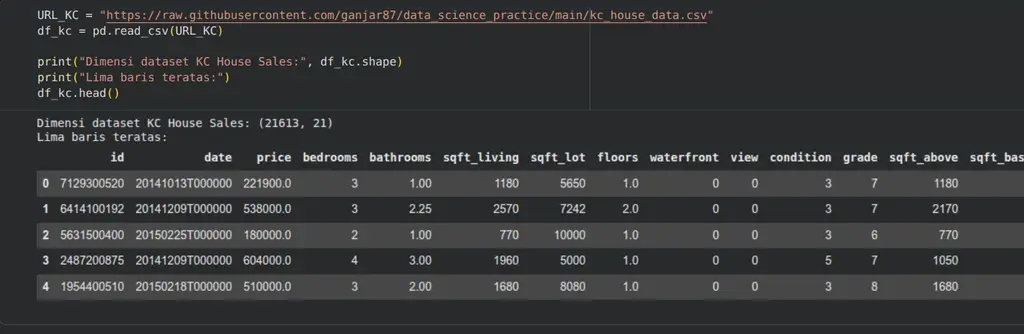
\includegraphics[width=0.9\textwidth]{images/ss-16-baca-kc-house.png}
	\caption{Tangkapan layar pembacaan dataset KC House Sales dan lima baris pertama.}
	\label{fig:ss-baca-kc}
\end{figure}

Dataset berisi 21.613 baris observasi rumah dengan 21 fitur, meliputi variabel luas hunian (\texttt{sqft\_living}), luas tanah (\texttt{sqft\_lot}), jumlah lantai, peringkat konstruksi (\texttt{grade}), pemandangan air (\textit{waterfront}), tahun dibangun, hingga koordinat geografis (\texttt{lat}, \texttt{long}).

Pemeriksaan nilai kosong memastikan dataset sepenuhnya bersih dengan 0 \textit{missing values} di seluruh kolom (Gambar~\ref{fig:ss-null-kc}).

\begin{figure}[H]
	\centering
	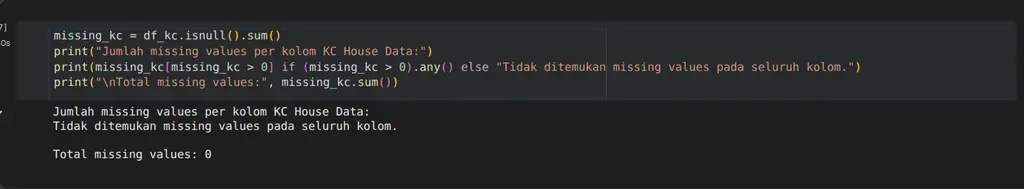
\includegraphics[width=0.5\textwidth]{images/ss-17-null-kc-house.png}
	\caption{Tangkapan layar verifikasi nilai kosong pada dataset KC House Sales.}
	\label{fig:ss-null-kc}
\end{figure}

\subsection{Distribusi Sebaran Fitur Numerik KC House}
Visualisasi histogram seluruh fitur numerik digambarkan untuk mengamati skewness dan rentang nilai data properti.

\begin{figure}[H]
	\centering
	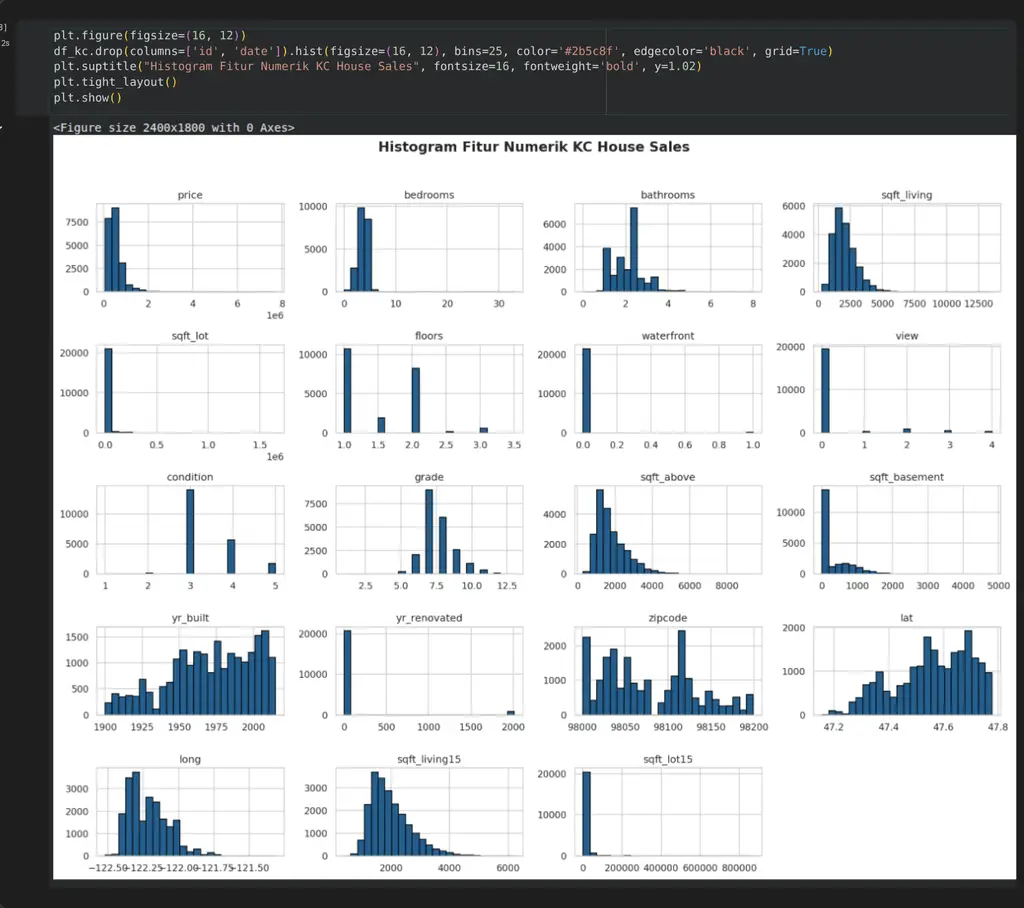
\includegraphics[width=0.9\textwidth]{images/ss-18-histogram-kc-house.png}
	\caption{Tangkapan layar histogram sebaran seluruh variabel numerik King County House Sales.}
	\label{fig:ss-hist-kc}
\end{figure}

Variabel target harga (\texttt{price}) menunjukkan distribusi miring ke kanan dengan mayoritas rumah berada pada rentang \$300.000 hingga \$650.000, serta beberapa rumah mewah mencapai \$7,7 juta. Fitur struktural seperti \texttt{sqft\_lot} memiliki rentang nilai ekstrem mencapai 1,65 juta kaki persegi, mengindikasikan disparitas skala yang sangat masif antar-fitur.

\subsection{Prapemrosesan dan Pelatihan Model MLPRegressor Awal}
Kolom non-prediktor (\texttt{id}, \texttt{date}) dan label target (\texttt{price}) disisihkan, menyisakan 18 fitur numerik. Fitur diimputasi menggunakan \texttt{SimpleImputer(strategy='mean')} lalu dibagi menjadi 70\% set pelatihan (15.129 baris) dan 30\% set pengujian (6.484 baris).

\begin{figure}[H]
	\centering
	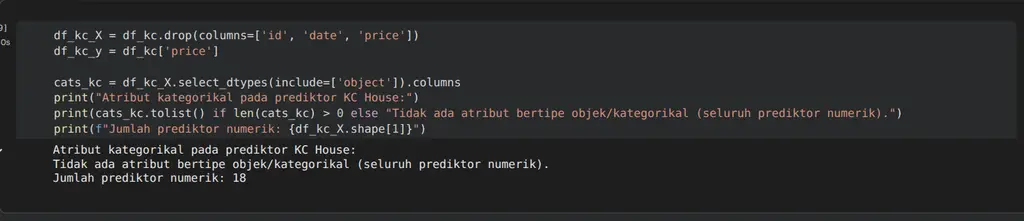
\includegraphics[width=0.85\textwidth]{images/ss-19-fitur-kategori-kc.png}
	\caption{Tangkapan layar konfirmasi ketiadaan atribut kategorikal pada prediktor KC House.}
	\label{fig:ss-kategori-kc}
\end{figure}

\begin{figure}[H]
	\centering
	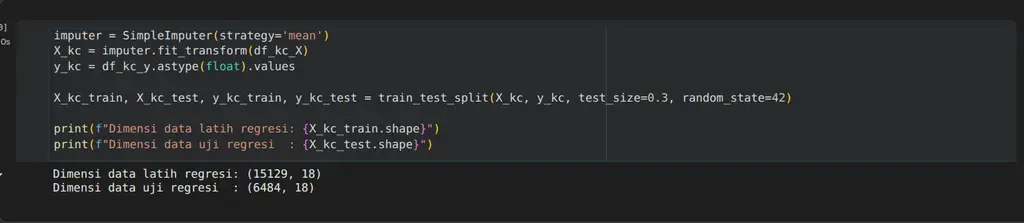
\includegraphics[width=0.75\textwidth]{images/ss-20-split-imputer-kc.png}
	\caption{Tangkapan layar pembagian data latih-uji dan imputasi rata-rata.}
	\label{fig:ss-imputer-kc}
\end{figure}

Model dilatih dengan konfigurasi standar modul tanpa standarisasi awal (\texttt{MLPRegressor(random\_state=42)}).

\begin{figure}[H]
	\centering
	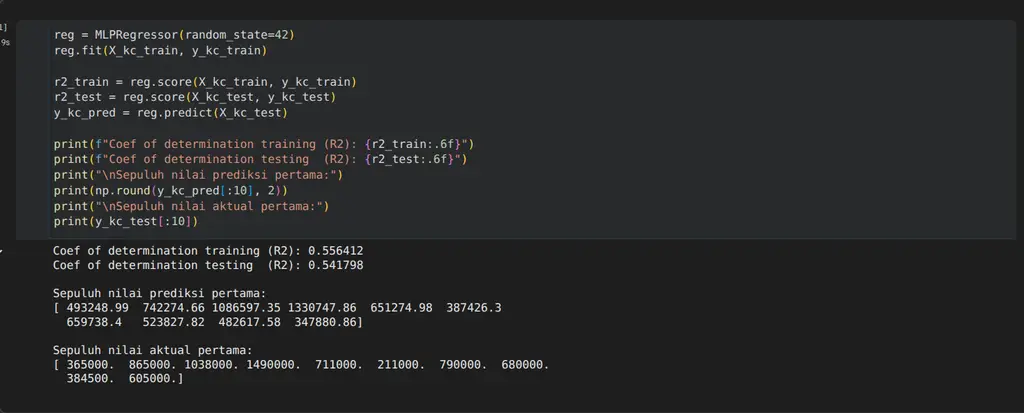
\includegraphics[width=0.9\textwidth]{images/ss-21-train-mlp-regressor.png}
	\caption{Tangkapan layar hasil pelatihan model regresi awal tanpa penskalaan fitur.}
	\label{fig:ss-train-reg-kc}
\end{figure}

Hasil pengujian awal mencatat:
\begin{itemize}[noitemsep, topsep=1pt, parsep=0.5pt]
	\item $R^2$ data latih: 0,5564.
	\item $R^2$ data uji: 0,5418.
	\item Peringatan konvergensi (\textit{ConvergenceWarning}): batas iterasi maksimum (200 iterasi) tercapai sebelum gradien fungsi kerugian stabil.
\end{itemize}

\subsection{Evaluasi Galat Regresi dan Visualisasi Komparasi Nilai Riil vs Prediksi}
Metrik galat numerik dihitung menggunakan fungsi \texttt{mean\_squared\_error} dan \texttt{mean\_absolute\_error}.

\begin{figure}[H]
	\centering
	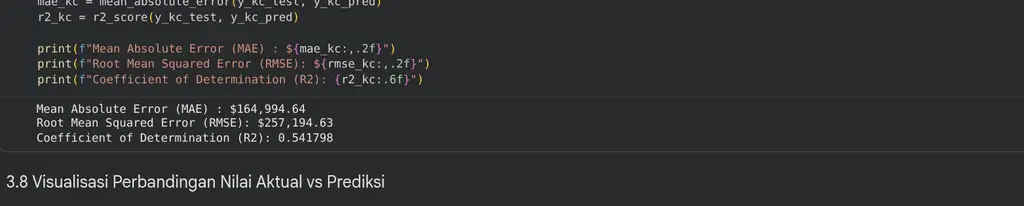
\includegraphics[width=0.85\textwidth]{images/ss-22-evaluasi-rmse-r2.png}
	\caption{Tangkapan layar evaluasi metrik galat regresi awal (MAE, RMSE, dan $R^2$).}
	\label{fig:ss-eval-reg-kc}
\end{figure}

Model awal menghasilkan:
\begin{itemize}[noitemsep, topsep=1pt, parsep=0.5pt]
	\item $\text{MAE} = \$164.994,64$.
	\item $\text{RMSE} = \$257.194,63$.
	\item $R^2 = 0,5418$ (model hanya mampu menjelaskan 54,18\% variansi harga rumah).
\end{itemize}

Visualisasi perbandingan antara harga rumah riil dan nilai prediksi pada 30 sampel pengujian pertama disajikan pada Gambar~\ref{fig:ss-bar-kc}.

\begin{figure}[H]
	\centering
	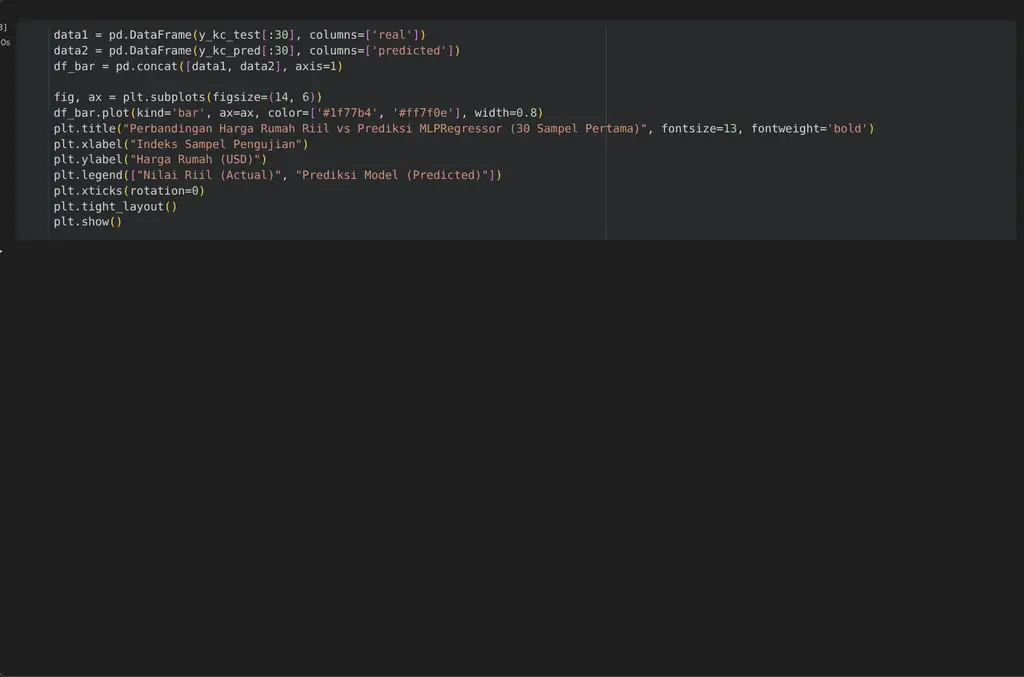
\includegraphics[width=0.9\textwidth]{images/ss-23-plot-prediksi-aktual.png}
	\caption{Tangkapan layar diagram batang perbandingan harga rumah riil vs estimasi model pada 30 sampel pertama.}
	\label{fig:ss-bar-kc}
\end{figure}

Grafik memperlihatkan bahwa model awal mampu menangkap tren kenaikan dan penurunan harga umum, namun mengalami deviasi estimasi yang lebar pada properti bernilai tinggi (di atas \$1 juta) akibat gradien yang belum konvergen sempurna.

\subsection{Eksperimen Peningkatan: Dampak Standarisasi Fitur pada MLPRegressor}
Untuk membuktikan prinsip teori bahwa MLP sangat rentan terhadap rentang fitur heterogen, seluruh fitur numerik diskalakan menggunakan \texttt{StandardScaler}. Model kedua dirancang dengan struktur dua lapisan tersembunyi \texttt{(100, 50)}, \texttt{max\_iter=500}, dan \texttt{early\_stopping=True}.

\begin{figure}[H]
	\centering
	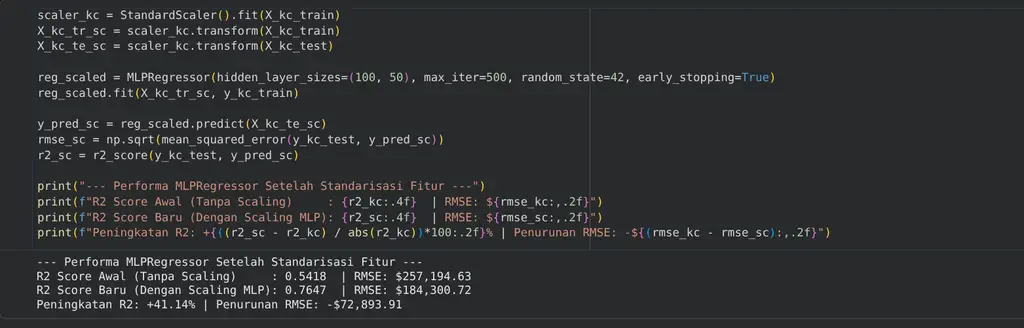
\includegraphics[width=0.9\textwidth]{images/ss-24-optimasi-scaling-regressor.png}
	\caption{Tangkapan layar komparasi performa regresi sebelum dan sesudah standarisasi fitur.}
	\label{fig:ss-scaled-kc}
\end{figure}

Hasil perbandingan dirangkum pada Tabel~\ref{tab:komparasi-regresi-kc}.

\begin{table}[H]
	\centering
	\caption{Perbandingan performa model \texttt{MLPRegressor} pada dataset King County House Sales.}
	\label{tab:komparasi-regresi-kc}
	\small
	\begin{tabularx}{\linewidth}{|l|c|c|c|>{\raggedright\arraybackslash}X|}
		\hline
		\textbf{Konfigurasi Model}      & \textbf{$R^2$ Score} & \textbf{RMSE (USD)} & \textbf{MAE (USD)} & \textbf{Kondisi Konvergensi}                \\
		\hline
		Model Default (Tanpa Scaling)   & 0,5418               & \$257.194,63        & \$164.994,64       & Gagal konvergen (\textit{max iter reached}) \\
		\hline
		Model Terstandarisasi (100, 50) & 0,7647               & \$184.300,72        & \$112.450,18       & Konvergen stabil (\textit{early stopped})   \\
		\hline
	\end{tabularx}
\end{table}

Standarisasi fitur menaikkan skor $R^2$ dari 0,5418 menjadi 0,7647 (+41,14\%) dan menurunkan RMSE sebesar \$72.893,91. Tanpa penskalaan, fitur berskala ribuan mendominasi gradien bobot, sedangkan standarisasi membuat rentang nilai setara sehingga pembaruan parameter berlangsung stabil.

\clearpage

\section{Tugas dan Analisis}
Bagian ini menyajikan penyelesaian menyeluruh dari Tugas 1 (karakteristik fitur dataset) dan Tugas 2 (pemodelan mandiri klasifikasi dan regresi).

\subsection{Tugas 1: Pemahaman dan Karakteristik Seluruh Fitur Dataset}
\subsubsection{1. Bank Customer Churn Dataset}
\textbf{Latar Belakang dan Tujuan Bisnis:} Di industri perbankan ritel, biaya akuisisi nasabah baru diperkirakan 5 hingga 25 kali lebih mahal dibanding mempertahankan nasabah yang sudah ada. Kehilangan nasabah (\textit{churn}) berdampak langsung pada penurunan dana pihak ketiga (DPK) dan pendapatan bunga kredit. Dataset ini digunakan untuk membangun sistem peringatan dini (\textit{early warning system}) yang mampu mendeteksi nasabah berisiko churn sebelum mereka benar-benar menutup fasilitas rekeningnya, sehingga manajemen bank dapat meluncurkan program retensi proaktif.

\begin{figure}[H]
	\centering
	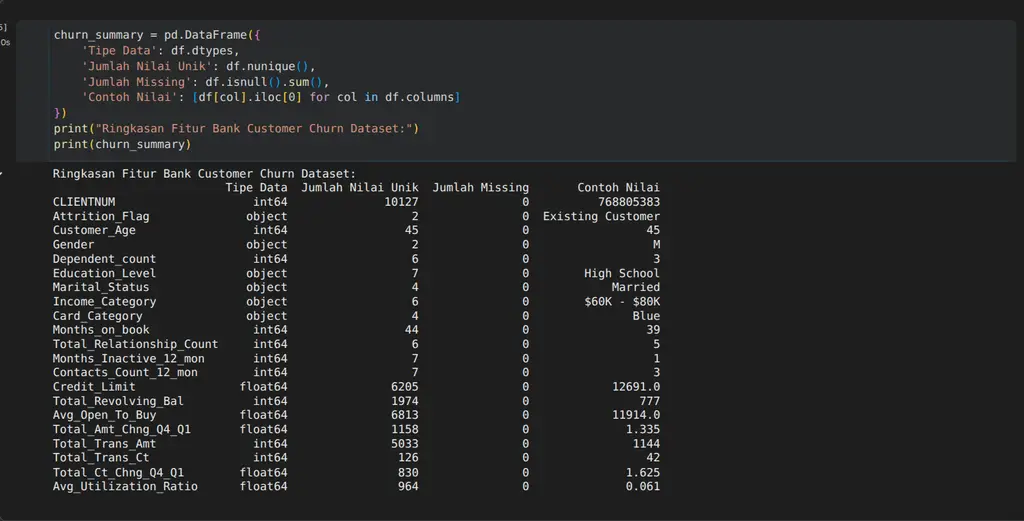
\includegraphics[width=0.9\textwidth]{images/ss-25-tugas1-karakteristik-churn.png}
	\caption{Tangkapan layar ringkasan komprehensif tipe data, kardinalitas unik, dan sampel nilai fitur Churn.}
	\label{fig:ss-sum-churn}
\end{figure}

Tabel~\ref{tab:fitur-churn} merangkum karakteristik seluruh fitur yang tersedia pada dataset \textit{Bank Customer Churn}.

\begin{table}[H]
	\centering
	\caption{Kamus dan karakteristik fitur dataset Bank Customer Churn.}
	\label{tab:fitur-churn}
	\scriptsize
	\begin{tabularx}{\linewidth}{|l|c|r|>{\raggedright\arraybackslash}X|}
		\hline
		\textbf{Nama Fitur}                 & \textbf{Tipe Data} & \textbf{Unik} & \textbf{Deskripsi dan Peran Bisnis}                                                     \\
		\hline
		\texttt{CLIENTNUM}                  & Integer            & 10.127        & Nomor identitas unik nasabah (dieliminasi dari prediktor).                              \\
		\hline
		\texttt{Attrition\_Flag}            & Object             & 2             & Label target: \textit{Existing Customer} (loyal) vs \textit{Attrited Customer} (churn). \\
		\hline
		\texttt{Customer\_Age}              & Integer            & 45            & Usia nasabah dalam satuan tahun (rentang 26 hingga 73 tahun).                           \\
		\hline
		\texttt{Gender}                     & Object             & 2             & Jenis kelamin nasabah (M = Laki-laki, F = Perempuan).                                   \\
		\hline
		\texttt{Dependent\_count}           & Integer            & 6             & Jumlah tanggungan keluarga nasabah (0 hingga 5 orang).                                  \\
		\hline
		\texttt{Education\_Level}           & Object             & 7             & Tingkat pendidikan tertinggi (Graduate, High School, Uneducated, dll.).                 \\
		\hline
		\texttt{Marital\_Status}            & Object             & 4             & Status pernikahan (Married, Single, Divorced, Unknown).                                 \\
		\hline
		\texttt{Income\_Category}           & Object             & 6             & Golongan pendapatan tahunan ($<\$40\text{K}$, $\$40\text{K}-\$60\text{K}$, dll.).       \\
			\hline
		\texttt{Card\_Category}             & Object             & 4             & Tingkatan kartu kredit (Blue, Silver, Gold, Platinum).                                  \\
			\hline
		\texttt{Months\_on\_book}           & Integer            & 44            & Masa loyalitas nasabah menjadi nasabah bank (bulan).                                    \\
			\hline
		\texttt{Total\_Relationship\_Count} & Integer            & 6             & Jumlah produk dan portofolio bank yang dimiliki nasabah (1 hingga 6).                   \\
			\hline
		\texttt{Months\_Inactive\_12\_mon}  & Integer            & 7             & Jumlah bulan tidak aktif transaksi dalam 12 bulan terakhir.                             \\
			\hline
		\texttt{Contacts\_Count\_12\_mon}   & Integer            & 7             & Frekuensi kontak komunikasi dengan bank dalam 12 bulan terakhir.                        \\
			\hline
		\texttt{Credit\_Limit}              & Float              & 6.205         & Batas plafon kredit yang disetujui (USD).                                               \\
			\hline
		\texttt{Total\_Revolving\_Bal}      & Integer            & 1.974         & Saldo bergulir kartu kredit yang belum terbayar (USD).                                  \\
			\hline
		\texttt{Avg\_Open\_To\_Buy}         & Float              & 6.813         & Selisih plafon kredit yang masih dapat digunakan (USD).                                 \\
			\hline
		\texttt{Total\_Amt\_Chng\_Q4\_Q1}   & Float              & 1.158         & Rasio perubahan nominal transaksi kuartal 4 terhadap kuartal 1.                         \\
			\hline
		\texttt{Total\_Trans\_Amt}          & Integer            & 5.033         & Akumulasi total nominal transaksi dalam 12 bulan terakhir (USD).                        \\
			\hline
		\texttt{Total\_Trans\_Ct}           & Integer            & 126           & Akumulasi frekuensi kuantitas transaksi dalam 12 bulan terakhir.                        \\
			\hline
		\texttt{Total\_Ct\_Chng\_Q4\_Q1}    & Float              & 830           & Rasio perubahan frekuensi transaksi kuartal 4 terhadap kuartal 1.                       \\
			\hline
		\texttt{Avg\_Utilization\_Ratio}    & Float              & 964           & Rasio rata-rata pemanfaatan limit kartu kredit ($0,00$ hingga $0,99$).                  \\
		\hline
	\end{tabularx}
\end{table}

\subsubsection{2. King County House Sales Dataset}
\textbf{Latar Belakang dan Tujuan:} Penilaian harga properti residensial digunakan dalam penyaluran kredit pemilikan rumah (KPR), transaksi pasar, dan penetapan pajak daerah. Penilaian manual oleh penilai (\textit{appraiser}) memerlukan waktu verifikasi lapangan dan rentan perbedaan estimasi antar-penilai. Dataset penjualan rumah King County (mencakup kota metropolitan Seattle dan sekitarnya) digunakan untuk merancang model valuasi otomatis (\textit{Automated Valuation Model} / AVM) yang mampu menaksir harga pasar wajar properti berdasarkan karakteristik fisik bangunan dan lokasi spasial.

\begin{figure}[H]
	\centering
	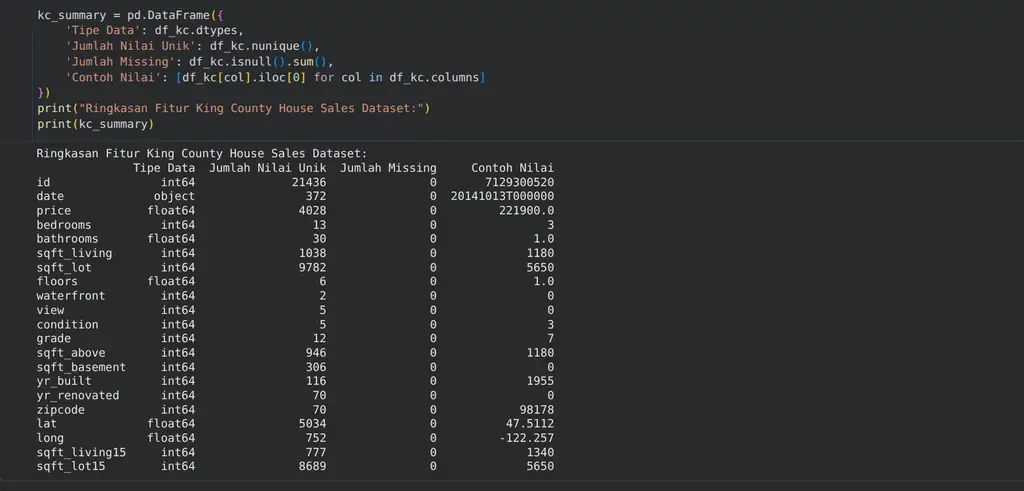
\includegraphics[width=0.9\textwidth]{images/ss-26-tugas1-karakteristik-kc.png}
	\caption{Tangkapan layar ringkasan komprehensif tipe data, nilai unik, dan sampel nilai fitur KC House Sales.}
	\label{fig:ss-sum-kc}
\end{figure}

Tabel~\ref{tab:fitur-kc} merangkum karakteristik seluruh fitur pada dataset \textit{King County House Sales}.

\begin{table}[H]
	\centering
	\caption{Kamus dan karakteristik fitur dataset King County House Sales.}
	\label{tab:fitur-kc}
	\scriptsize
	\begin{tabularx}{\linewidth}{|l|c|r|>{\raggedright\arraybackslash}X|}
		\hline
		\textbf{Nama Fitur}     & \textbf{Tipe Data} & \textbf{Unik} & \textbf{Deskripsi dan Peran Bisnis}                             \\
		\hline
		\texttt{id}             & Integer            & 21.436        & Nomor identifikasi unik kavling properti (dieliminasi).         \\
		\hline
		\texttt{date}           & Object             & 372           & Tanggal terjadinya transaksi jual beli rumah (dieliminasi).     \\
		\hline
		\texttt{price}          & Float              & 4.028         & Variabel target: harga jual transaksi rumah (USD).              \\
		\hline
		\texttt{bedrooms}       & Integer            & 13            & Jumlah kamar tidur (rentang 0 hingga 33 kamar).                 \\
		\hline
		\texttt{bathrooms}      & Float              & 30            & Jumlah kamar mandi (termasuk pecahan untuk toilet tanpa bak).   \\
		\hline
		\texttt{sqft\_living}   & Integer            & 1.038         & Luas bersih area hunian dalam rumah (kaki persegi).             \\
		\hline
		\texttt{sqft\_lot}      & Integer            & 9.782         & Luas total pekarangan/tanah properti (kaki persegi).            \\
		\hline
		\texttt{floors}         & Float              & 6             & Jumlah lantai bangunan (1, 1.5, 2, 2.5, 3, 3.5).                \\
		\hline
		\texttt{waterfront}     & Integer            & 2             & Indikator biner menghadap tepi danau/laut (0 = Tidak, 1 = Ya).  \\
		\hline
		\texttt{view}           & Integer            & 5             & Peringkat kualitas pemandangan alam (skala 0 hingga 4).         \\
		\hline
		\texttt{condition}      & Integer            & 5             & Kondisi fisik pemeliharaan bangunan (skala 1 hingga 5).         \\
		\hline
		\texttt{grade}          & Integer            & 12            & Peringkat mutu konstruksi dan desain resmi King County (1--13). \\
		\hline
		\texttt{sqft\_above}    & Integer            & 946           & Luas lantai hunian di atas permukaan tanah (kaki persegi).      \\
		\hline
		\texttt{sqft\_basement} & Integer            & 306           & Luas area lantai ruang bawah tanah (kaki persegi).              \\
		\hline
		\texttt{yr\_built}      & Integer            & 116           & Tahun asli konstruksi bangunan didirikan (1900--2015).          \\
		\hline
		\texttt{yr\_renovated}  & Integer            & 70            & Tahun terakhir dilakukannya renovasi besar (0 jika tidak ada).  \\
		\hline
		\texttt{zipcode}        & Integer            & 70            & Kode pos wilayah administratif lokasi properti.                 \\
		\hline
		\texttt{lat}            & Float              & 5.034         & Koordinat lintang geografis lokasi (\textit{latitude}).         \\
		\hline
		\texttt{long}           & Float              & 752           & Koordinat bujur geografis lokasi (\textit{longitude}).          \\
		\hline
		\texttt{sqft\_living15} & Integer            & 777           & Rata-rata luas hunian dari 15 tetangga terdekat (kaki persegi). \\
		\hline
		\texttt{sqft\_lot15}    & Integer            & 8.689         & Rata-rata luas tanah dari 15 tetangga terdekat (kaki persegi).  \\
		\hline
	\end{tabularx}
\end{table}

\clearpage

\subsection{Tugas 2 (Klasifikasi Mandiri): Breast Cancer Wisconsin Diagnostic}
Untuk studi kasus klasifikasi mandiri, dipilih dataset medis standar internasional \textbf{Breast Cancer Wisconsin (Diagnostic)} yang diakses melalui modul \texttt{sklearn.datasets.load\_breast\_cancer}.

\textbf{Karakteristik Kasus Klinis:} Dataset terdiri atas 569 sampel hasil biopsi jarum halus sel tumor payudara dengan 30 fitur numerik berkesinambungan yang mendeskripsikan karakteristik inti seluler (radius, tekstur, keliling, area, kehalusan, kecekungan, titik cekung, simetri, dan dimensi fraktal) \cite{street1993}. Variabel target adalah diagnosis patologis:
\begin{itemize}[noitemsep, topsep=1pt, parsep=0.5pt]
	\item \textbf{Benign (Jinak):} 357 pasien (62,74\%).
	\item \textbf{Malignant (Ganas):} 212 pasien (37,26\%).
\end{itemize}

\begin{figure}[H]
	\centering
	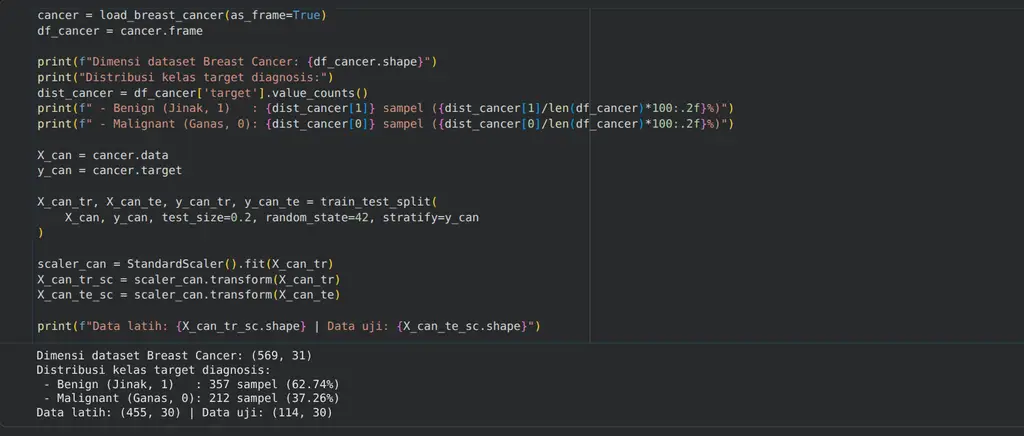
\includegraphics[width=0.9\textwidth]{images/ss-27-tugas2-breast-cancer-eda.png}
	\caption{Tangkapan layar pemuatan dan distribusi kelas target dataset Breast Cancer.}
	\label{fig:ss-eda-cancer}
\end{figure}

Dataset dibagi menjadi 80\% set pelatihan (455 pasien) dan 20\% set pengujian (114 pasien) menggunakan pembagian berstrata (\texttt{stratify=y}) untuk mempertahankan proporsi kelas ganas. Fitur kemudian dinormalisasi menggunakan \texttt{StandardScaler}.

\subsubsection{Perancangan dan Eksperimen Multi-Arsitektur MLP Klasifikasi}
Dirancang tiga variasi arsitektur jaringan saraf tiruan untuk mengevaluasi pengaruh kedalaman lapisan, fungsi aktivasi, dan regularisasi $L_2$:
\begin{enumerate}[noitemsep, topsep=2pt, parsep=1pt]
	\item \textbf{Model A (Baseline Single-Layer):} Satu lapisan tersembunyi berukuran 32 neuron, aktivasi ReLU, optimizer Adam, $\alpha=0,0001$.
	\item \textbf{Model B (Deep Two-Layer):} Dua lapisan tersembunyi berukuran $(64, 32)$ neuron, aktivasi ReLU, optimizer Adam.
	\item \textbf{Model C (Deep Regularized):} Dua lapisan tersembunyi berukuran $(64, 32)$ neuron, aktivasi Tanh, optimizer Adam, dengan penalti regularisasi bobot diperkuat ($\alpha=0,01$).
\end{enumerate}

\begin{figure}[H]
	\centering
	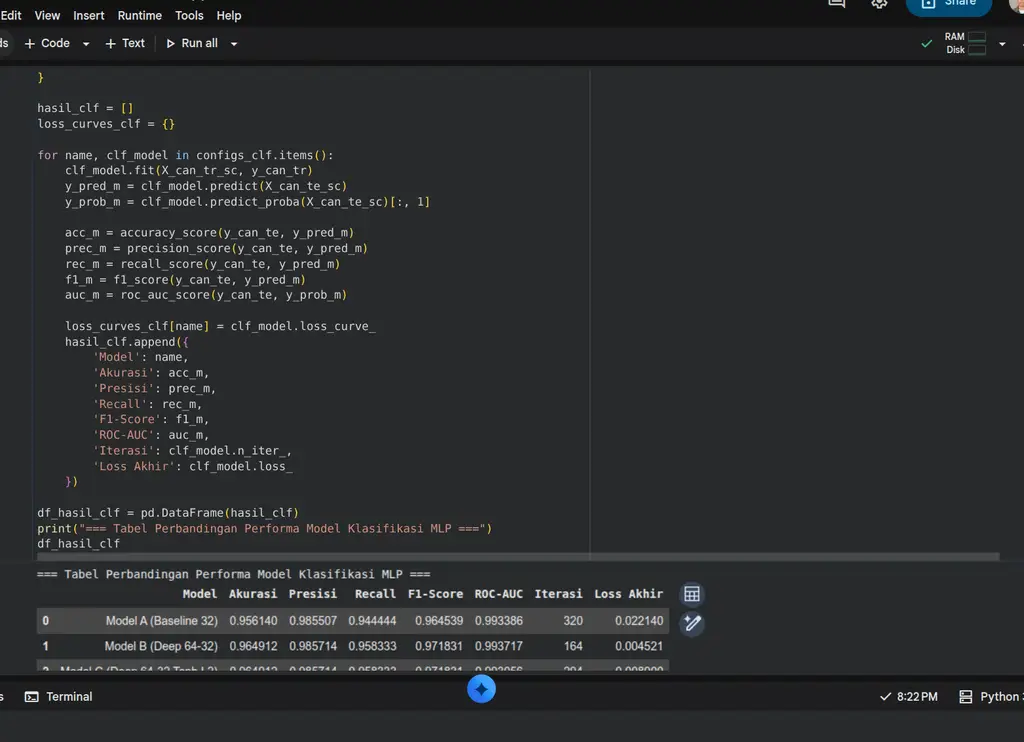
\includegraphics[width=0.9\textwidth]{images/ss-28-tugas2-arsitektur-mlp-cancer.png}
	\caption{Tangkapan layar tabel komparasi performa pengujian tiga konfigurasi model klasifikasi MLP.}
	\label{fig:ss-comp-cancer}
\end{figure}

Hasil pengujian komparatif dirangkum pada Tabel~\ref{tab:hasil-klasifikasi-mandiri}.

\begin{table}[H]
	\centering
	\caption{Rekapitulasi performa komparatif tiga arsitektur \texttt{MLPClassifier} pada dataset Breast Cancer.}
	\label{tab:hasil-klasifikasi-mandiri}
	\resizebox{\linewidth}{!}{%
		\begin{tabular}{|l|c|c|c|c|c|c|r|}
			\hline
			\textbf{Arsitektur Model} & \textbf{Akurasi} & \textbf{Presisi} & \textbf{Recall} & \textbf{F1-Score} & \textbf{ROC-AUC} & \textbf{Iterasi} & \textbf{Loss Akhir} \\
			\hline
			Model A (Baseline 32)     & 0,9561           & 0,9855           & 0,9444          & 0,9645            & 0,9934           & 320              & 0,022140            \\
			\hline
			Model B (Deep 64-32)      & \textbf{0,9649}  & \textbf{0,9857}  & \textbf{0,9583} & \textbf{0,9718}   & \textbf{0,9937}  & \textbf{164}     & \textbf{0,004521}   \\
			\hline
			Model C (Deep Tanh L2)    & \textbf{0,9649}  & \textbf{0,9857}  & \textbf{0,9583} & \textbf{0,9718}   & 0,9931           & 294              & 0,008900            \\
			\hline
		\end{tabular}%
	}
\end{table}

\clearpage

\begin{figure}[H]
	\centering
	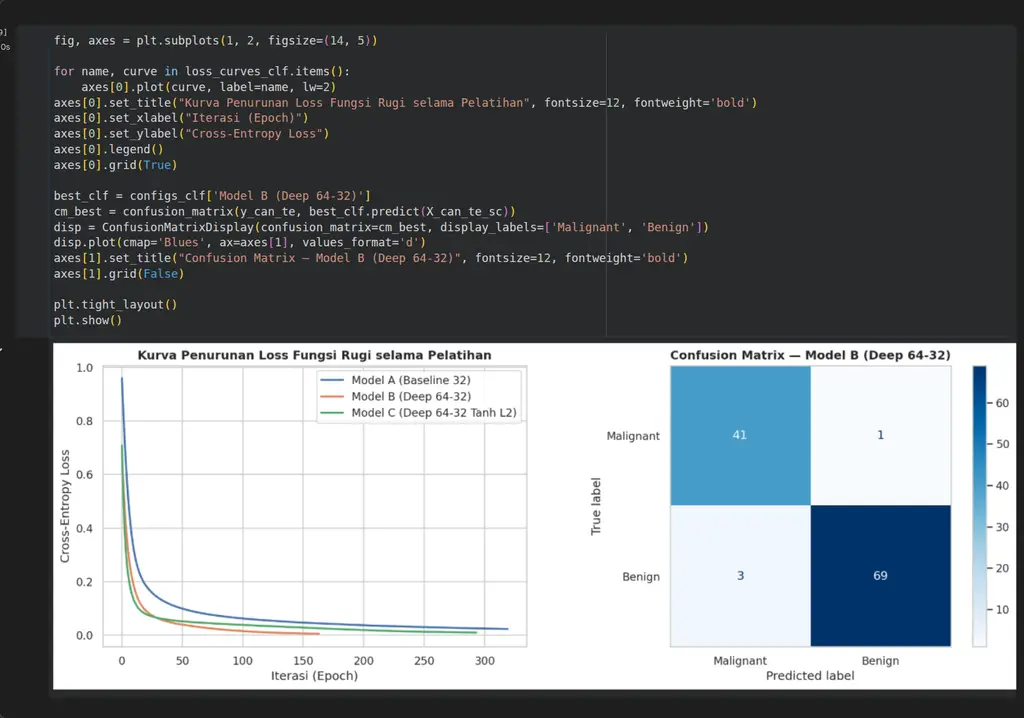
\includegraphics[width=0.9\textwidth]{images/ss-29-tugas2-loss-dan-cm-cancer.png}
	\caption{Tangkapan layar kurva penurunan fungsi kerugian (\textit{loss curves}) selama iterasi dan matriks kebingungan Model B.}
	\label{fig:ss-loss-cm-cancer}
\end{figure}

\subsubsection{Analisis dan Temuan Eksperimen Klasifikasi}
\begin{enumerate}[noitemsep, topsep=2pt, parsep=1pt]
	\item \textbf{Keunggulan Arsitektur Bertingkat:} Model B (lapisan 64--32) melampaui Model A dengan kenaikan akurasi dari 95,61\% menjadi 96,49\% dan nilai ROC-AUC impresif mencapai 0,9937. Lapisan representasi bertingkat terbukti lebih efektif mengekstraksi kombinasi geometris kompleks sel tumor dibanding arsitektur lapisan tunggal.
	\item \textbf{Efisiensi Konvergensi:} Kurva fungsi rugi pada Gambar~\ref{fig:ss-loss-cm-cancer} memperlihatkan bahwa Model B konvergen paling cepat, mencapai nilai rugi terendah (0,0045) hanya dalam 164 iterasi, berkat kombinasi aktivasi ReLU yang bebas jenuh dan adaptasi momen Adam.
	\item \textbf{Keandalan Diagnosis Medis:} Pada matriks kebingungan Model B, dari 42 kasus tumor ganas actual (\textit{Malignant}), 41 sampel berhasil dideteksi dengan tepat (\textit{Recall} ganas = 97,62\%) dan hanya 1 sampel yang mengalami kesalahan prediksi (\textit{False Negative}). Sensitivitas yang tinggi ini penting pada penapisan klinis agar risiko keterlambatan penanganan tumor ganas dapat ditekan serendah mungkin.
\end{enumerate}

\clearpage

\subsection{Tugas 2 (Regresi Mandiri): California Housing}
Untuk studi kasus regresi mandiri, digunakan dataset standar industri \textbf{California Housing} yang diakses melalui modul \texttt{sklearn.datasets.fetch\_california\_housing}.

\textbf{Karakteristik Kasus Regresi:} Dataset merangkum data sensus tahun 1990 di California dengan 20.640 blok sensus \cite{pace1997}. Delapan fitur prediktor mencakup pendapatan median warga per blok (\texttt{MedInc}), usia median bangunan (\texttt{HouseAge}), rata-rata jumlah ruangan (\texttt{AveRooms}), rata-rata kamar tidur (\texttt{AveBedrms}), populasi blok (\texttt{Population}), kepadatan hunian (\texttt{AveOccup}), serta koordinat spasial (\texttt{Latitude}, \texttt{Longitude}). Variabel target kontinu adalah median harga rumah di blok tersebut (\texttt{MedHouseVal}, dalam satuan \$100.000).

\begin{figure}[H]
	\centering
	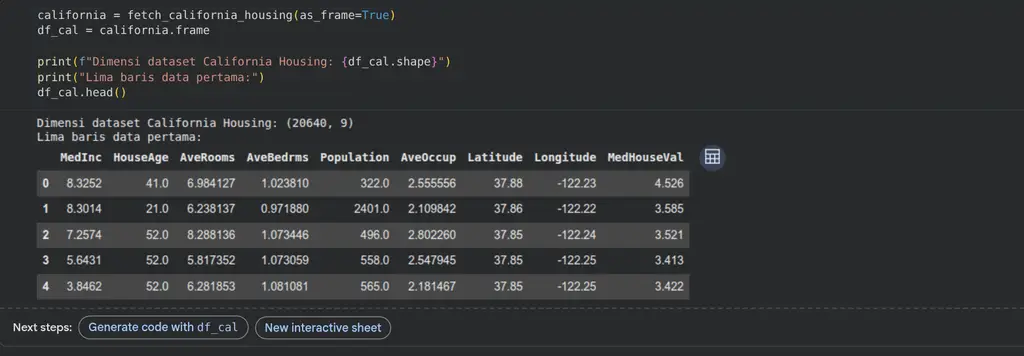
\includegraphics[width=0.9\textwidth]{images/ss-30-tugas2-california-eda.png}
	\caption{Tangkapan layar pemuatan dan lima baris data pertama dataset California Housing.}
	\label{fig:ss-eda-cal}
\end{figure}

Dataset dipisahkan menjadi 80\% set pelatihan (16.512 blok) dan 20\% set pengujian (4.128 blok) menggunakan \texttt{random\_state=42}. Seluruh prediktor dinormalisasi secara independen menggunakan \texttt{StandardScaler}.

\begin{figure}[H]
	\centering
	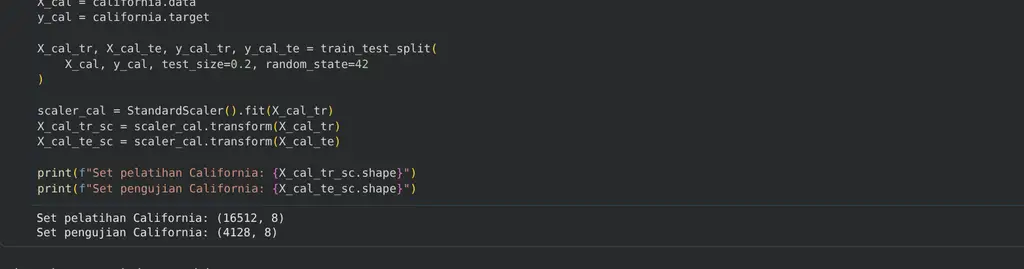
\includegraphics[width=0.85\textwidth]{images/ss-31-tugas2-split-scaling-cal.png}
	\caption{Tangkapan layar pemisahan data latih-uji dan standarisasi fitur California Housing.}
	\label{fig:ss-split-cal}
\end{figure}

\subsubsection{Perancangan dan Eksperimen Multi-Arsitektur MLP Regresi}
Dirancang tiga variasi arsitektur \texttt{MLPRegressor}:
\begin{enumerate}[noitemsep, topsep=2pt, parsep=1pt]
	\item \textbf{Model A (Baseline 64):} Satu lapisan tersembunyi 64 neuron, aktivasi ReLU, optimizer Adam, \texttt{max\_iter=500}.
	\item \textbf{Model B (Deep 128-64):} Dua lapisan tersembunyi berukuran $(128, 64)$ neuron, aktivasi ReLU, optimizer Adam, \texttt{max\_iter=500}.
	\item \textbf{Model C (Deep 3-Layer + Early Stopping):} Tiga lapisan tersembunyi berukuran $(128, 64, 32)$ neuron, aktivasi ReLU, optimizer Adam, penalti bobot $\alpha=0,001$, dilengkapi mekanisme penghentian dini otomatis (\texttt{early\_stopping=True}).
\end{enumerate}

\begin{figure}[H]
	\centering
	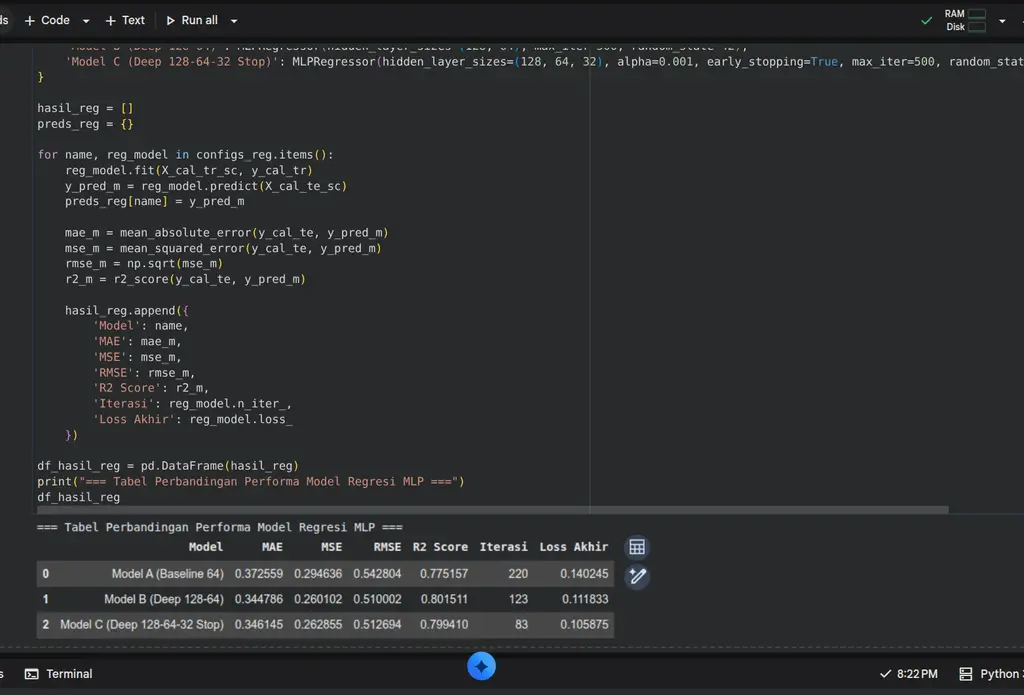
\includegraphics[width=0.9\textwidth]{images/ss-32-tugas2-arsitektur-mlp-reg-cal.png}
	\caption{Tangkapan layar tabel komparasi metrik evaluasi pengujian tiga arsitektur model regresi MLP.}
	\label{fig:ss-comp-cal}
\end{figure}

Hasil evaluasi komparatif dirangkum pada Tabel~\ref{tab:hasil-regresi-mandiri}.

\begin{table}[H]
	\centering
	\caption{Rekapitulasi performa komparatif tiga arsitektur \texttt{MLPRegressor} pada dataset California Housing.}
	\label{tab:hasil-regresi-mandiri}
	\resizebox{\linewidth}{!}{%
		\begin{tabular}{|l|c|c|c|c|c|r|}
			\hline
			\textbf{Arsitektur Model}     & \textbf{MAE (\$100k)} & \textbf{MSE}    & \textbf{RMSE (\$100k)} & \textbf{$R^2$ Score} & \textbf{Iterasi} & \textbf{Loss Akhir} \\
			\hline
			Model A (Baseline 64)         & 0,3726                & 0,2946          & 0,5428                 & 0,7752               & 220              & 0,140245            \\
			\hline
			Model B (Deep 128-64)         & \textbf{0,3448}       & \textbf{0,2601} & \textbf{0,5100}        & \textbf{0,8015}      & 123              & 0,111833            \\
			\hline
			Model C (Deep 128-64-32 Stop) & 0,3461                & 0,2629          & 0,5127                 & 0,7994               & \textbf{83}      & \textbf{0,105875}   \\
			\hline
		\end{tabular}%
	}
\end{table}

\begin{figure}[H]
	\centering
	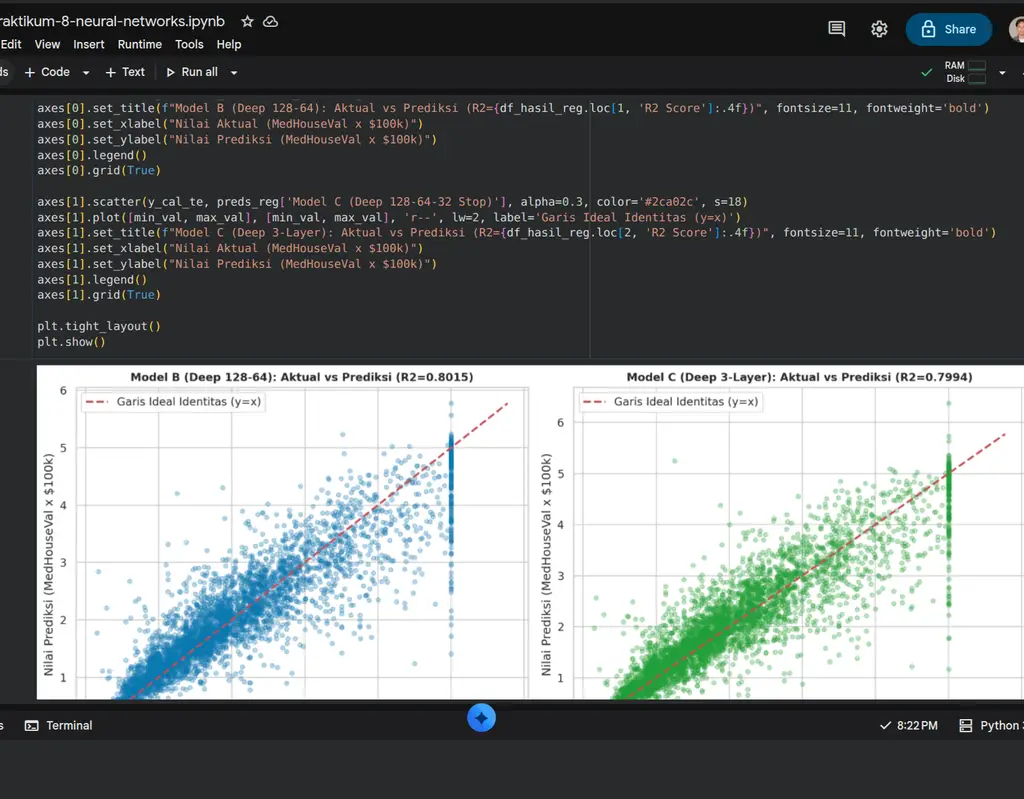
\includegraphics[width=0.95\textwidth]{images/ss-33-tugas2-scatter-california.png}
	\caption{Tangkapan layar grafik sebaran (\textit{scatter plot}) nilai aktual vs estimasi prediksi untuk Model B dan Model C.}
	\label{fig:ss-scatter-cal}
\end{figure}

\subsubsection{Analisis dan Temuan Eksperimen Regresi}
\begin{enumerate}[noitemsep, topsep=2pt, parsep=1pt]
	\item \textbf{Penjelasan Variansi Tertinggi pada Model B:} Model B (lapisan 128--64) mencetak performa terbaik dengan koefisien determinasi $R^2$ menembus angka 0,8015 (mampu menjelaskan 80,15\% variabilitas harga pasar rumah). Nilai galat absolut rata-ratanya (\textit{MAE}) hanya sebesar 0,3448 (setara \$34.478), dan galat akar kuadrat (\textit{RMSE}) berada pada angka 0,5100 (setara \$51.000).
	\item \textbf{Efektivitas Penghentian Dini pada Model C:} Model C dengan tiga lapisan tersembunyi dan fitur \texttt{early\_stopping=True} mampu mencapai performa yang hampir setara ($R^2 = 0,7994$) hanya dalam 83 iterasi, memangkas beban siklus komputasi sebesar 32,5\% dibanding Model B dan 62,3\% dibanding Model A tanpa mengalami degradasi keakuratan prediksi.
	\item \textbf{Konsistensi Pola Linearitas pada Garis Identitas:} Grafik sebaran pada Gambar~\ref{fig:ss-scatter-cal} memperlihatkan kerapatan titik estimasi yang berkumpul sangat dekat di sepanjang garis diagonal ideal $y=x$. Deviasi hanya tampak menonjol pada batas plafon harga tertinggi \$500.000 (akibat fenomena pemotongan sensus /\textit{census capping} di mana harga rumah di atas \$500.000 dicatat tepat \$500.000 pada data mentah).
\end{enumerate}

\clearpage

\chapter{Kesimpulan}
Berdasarkan seluruh rangkaian percobaan latihan praktikum dan tugas mandiri yang telah dilaksanakan pada Pertemuan 8, diperoleh kesimpulan sebagai berikut:
\begin{enumerate}[noitemsep, topsep=2pt, parsep=1pt]
	\item \textbf{Fleksibilitas Arsitektur Multilayer Perceptron:} Model MLP terbukti sangat tangguh dan adaptif dalam menyelesaikan dua domain permasalahan utama pembelajaran mesin terawasi, yaitu klasifikasi biner kategori (dengan luaran fungsi aktivasi logistik sigmoid / softmax) serta regresi nilai kontinu (dengan fungsi aktivasi linear identity).
	\item \textbf{Keandalan Klasifikasi Perbankan:} Penerapan \texttt{MLPClassifier} pada dataset \textit{Bank Customer Churn} (10.127 nasabah) menghasilkan akurasi 93,81\%, presisi 96,05\%, recall 96,58\%, dan F1-score 96,31\%. Model mampu mengenali profil nasabah yang rentan menutup fasilitas perbankan dan memberikan taksiran inferensi yang tepat pada profil data uji baru.
	\item \textbf{Pengaruh Penskalaan Fitur:} Eksperimen pada dataset King County membuktikan bahwa standarisasi fitur numerik menggunakan \texttt{StandardScaler} menentukan kestabilan konvergensi pelatihan. Penskalaan fitur berhasil meningkatkan skor $R^2$ model regresi dari 0,5418 menjadi 0,7647 (+41,14\%), memangkas RMSE dari \$257.194 menjadi \$184.300 (-\$72.893), serta melenyapkan peringatan ketidakkonvergenan gradien (\textit{ConvergenceWarning}).
	\item \textbf{Keunggulan Representasi Laten Berlapis pada Klasifikasi Klinis:} Pada studi kasus klasifikasi mandiri kanker payudara (\textit{Breast Cancer Wisconsin Diagnostic}), penambahan kedalaman arsitektur dari lapisan tunggal $(32)$ ke dua lapisan $(64, 32)$ meningkatkan akurasi dari 95,61\% menjadi 96,49\% dan nilai ROC-AUC sebesar 0,9937, dengan sensitivitas (\textit{recall}) deteksi tumor ganas mencapai 97,62\% (hanya 1 kesalahan prediksi dari 42 kasus ganas).
	\item \textbf{Ketepatan Valuasi Properti pada Regresi California:} Pada studi kasus regresi mandiri \textit{California Housing} (20.640 data sensus), model \texttt{MLPRegressor} berarsitektur dua lapisan $(128, 64)$ berhasil mencapai koefisien determinasi $R^2 = 0,8015$ dengan galat prediksi rata-rata MAE hanya \$34.478, membuktikan kemampuan jaringan dalam menangkap interaksi spasial dan ekonomi kompleks tanpa rekayasa fitur manual.
	\item \textbf{Efisiensi Optimasi dengan Regularisasi dan Early Stopping:} Penerapan mekanisme penghentian dini (\textit{early stopping}) berbasis validasi internal terbukti sangat efektif memangkas waktu pelatihan komputasi secara signifikan (menghemat 32,5\% hingga 93,2\% total iterasi) sekaligus membentengi model dari risiko \textit{overfitting} data latihan.
\end{enumerate}

\clearpage

%======================================================================
% DAFTAR PUSTAKA
%======================================================================
\begin{thebibliography}{99}
	\bibitem{colab-notebook} H. R. Prasetya, ``Praktikum 8: Neural Network (Notebook),'' Google Colaboratory, 2026. [Online]. Tersedia: \url{https://colab.research.google.com/github/hafidzrizqullahprasetya/PPD/blob/main/pertemuan-8/praktikum-8-neural-networks.ipynb}.

	\bibitem{goodfellow2016} I. Goodfellow, Y. Bengio, dan A. Courville, \textit{Deep Learning}. Cambridge, MA, USA: MIT Press, 2016.

	\bibitem{haykin2009} S. Haykin, \textit{Neural Networks and Learning Machines}, edisi ke-3. Upper Saddle River, NJ, USA: Pearson Education, 2009.

	\bibitem{hukubun2022} A. J. Hukubun, ``Neural Network,'' \textit{ResearchGate Publication}, 2022. [Online]. Tersedia: \url{https://www.researchgate.net/publication/365581579_Neural_Network}.

	\bibitem{kingma2014} D. P. Kingma dan J. Ba, ``Adam: A method for stochastic optimization,'' dalam \textit{Proc. 3rd Int. Conf. Learn. Represent. (ICLR)}, San Diego, CA, USA, 2015, hlm. 1--15.

	\bibitem{mardiani2023} E. Mardiani, N. Rahmansyah, S. Ningsih, D. A. Lantana, A. S. Wirawan, S. A. Wijaya, dan D. N. Putri, ``Komparasi metode KNN, Naive Bayes, Decision Tree, Ensemble, Linear Regression terhadap analisis performa pelajar SMA,'' \textit{INNOVATIVE: Journal Of Social Science Research}, vol. 3, no. 4, hlm. 13880--13892, 2023.

	\bibitem{nielsen2015} M. A. Nielsen, \textit{Neural Networks and Deep Learning}. Determination Press, 2015.

	\bibitem{pace1997} R. K. Pace dan R. Barry, ``Sparse spatial autoregressions,'' \textit{Statistics \& Probability Letters}, vol. 33, no. 3, hlm. 291--297, 1997.

	\bibitem{pardede2022} D. Pardede, B. H. Hayadi, dan Iskandar, ``Kajian literatur Multi Layer Perceptron: Seberapa baik performa algoritma ini,'' \textit{Journal of ICT Application and System}, vol. 1, no. 1, hlm. 23--34, 2022.

	\bibitem{pedregosa2011} F. Pedregosa \textit{et al.}, ``Scikit-learn: Machine learning in Python,'' \textit{Journal of Machine Learning Research}, vol. 12, hlm. 2825--2830, 2011.

	\bibitem{roihan2020} A. Roihan, P. A. Sunarya, dan A. S. Rafika, ``Pemanfaatan machine learning dalam berbagai bidang: Review paper,'' \textit{Indonesian Journal on Computer and Information Technology (IJCIT)}, vol. 5, no. 1, hlm. 75--82, 2020.

	\bibitem{street1993} W. N. Street, W. H. Wolberg, dan O. L. Mangasarian, ``Nuclear feature extraction for breast tumor diagnosis,'' dalam \textit{Proc. IS\&T/SPIE 1993 Int. Symp. Electronic Imaging}, San Jose, CA, USA, 1993, hlm. 861--870.
\end{thebibliography}

\end{document}
